\chapter{Theoretical Background}
\label{chap:2_background}

% VAE
% PPO
% 15pages

In this chapter, we will cover the relevant theory required to understand our two-part model, namely a \textit{Variational Autoencoder} (VAE) combined with a reinforcement learning agent -- a multi-layer perceptron (MLP) -- trained with \textit{Proximal Policy Optimisation} (PPO). 

First, a gentle introduction of \textit{unsupervised learning} will be given, along with its use in representation learning. Then, we will look into \textit{autoencoders} as a way of extracting features in a dataset before finally exploring the theory behind VAEs.
Later, in section \ref{sec:2_RL}, we will begin with a recollection of fundamental reinforcement learning concepts such as Markov Decision Processes, returns, value functions and policies. This will serve as a stepping stone to understanding the topic of policy optimisation, particularly \textit{actor-critics} and how PPO builds on this.


\section{Unsupervised Learning}
\label{sec:2_unsupervised_learning}
Machine learning algorithms are broadly classed into four categories: supervised, semi-supervised, unsupervised and reinforcement learning -- depending on what kind of experience the algorithms are allowed to have during the learning process. 
Though supervised learning has been one of the most powerful tools of AI, it requires labour-intensive feature engineering and labelling in order to create datasets in areas such as vision, audio and text \cite{LectureNotesSparseAutoencoder}. In contrast, unsupervised techniques learn from \textit{unlabelled} datasets, where, in a deep learning context, the aim is to learn the useful properties of the structure of this dataset or even its underlying probability distribution \cite{DeepLearningBook}.
The key idea is that by learning the useful properties of our data, we can use this as a better, more compact \textit{representation} of our input, significantly reducing its complexity.


\section{Representation Learning}
\label{sec:2_representation_learning}
Representation learning refers to the unsupervised learning of a dataset's useful structures or probability distribution in order to make a subsequent learning task easier \cite{DeepLearningBook}.
In \cite{RepresentationLearning2012}, it is highlighted that ``the performance of machine learning methods is heavily dependant on the choice of data representation,'' and that to ``understand the world around us,'' it must ``learn to identify and disentangle the underlying explanatory factors hidden in low-level sensory data.''
To explore these ideas, we focus on the use of autoencoders and variational autoencoders as a means of \textit{learning a representation} of a dataset.


\subsection{Autoencoders}
\label{subsec:2_autoencoders}
Autoencoders are a class of neural networks whose learning objective is an identity mapping from input to output, under some specific constraint \cite{NLPCA_autoencoder1991}. 
The mapping is described with two parts, first a function to describe an encoding $\bz = f(\bx)$, and then a function to describe a decoding $\br = g(\bz)$.
\begin{figure}[hbt]
    \centering
    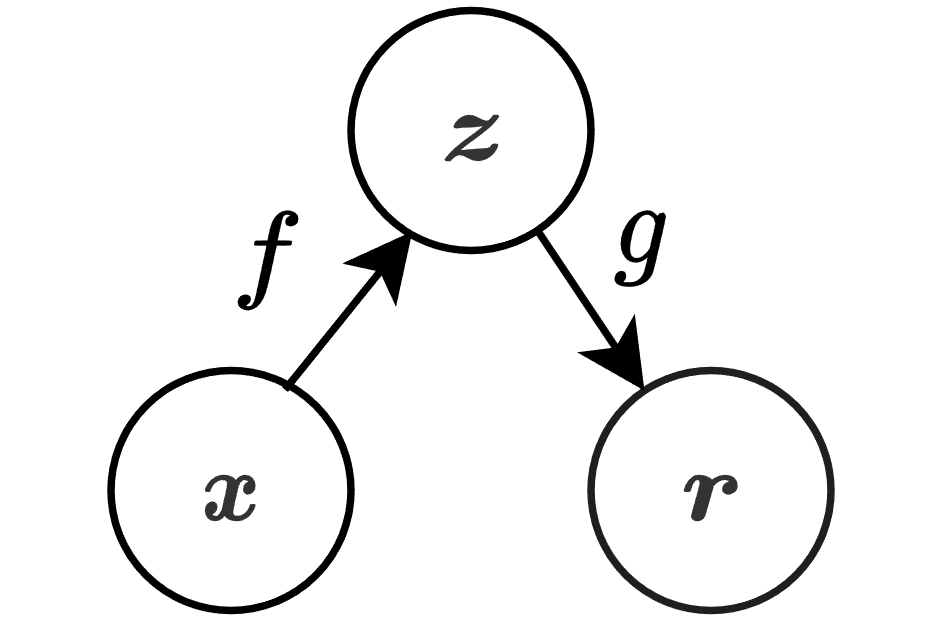
\includegraphics[width=0.3\textwidth]{figures/2_/2_general_autoencoder.png}
    \captionsetup{justification=centering}
    \caption{The general structure of an autoencoder showing how an input $\bx$ is encoded into a latent code $\bz$, before being mapped to a reconstruction $\br$ \cite{DeepLearningBook}.}
    \label{fig:2_general_autoencoder}
\end{figure}
Here, $\bx$ refers to the input data, while $\bz$ is the hidden layer of a neural network that represents a \textit{code} or \textit{latent representation}, and $\br$ is the reconstructed input mapped from the code $\bz$.

The constraint on an autoencoder is typically placed through its \textit{architectural design} or its \textit{learning process}, where the idea is to restrict autoencoders to prioritise only parts of the information in the input when reconstructing the input (mapping $\bx$ to $\bz$ and $\bz$ to $\br$). By doing so, the prioritised parts of the input will become a more useful, alternative representation of the input $\bx$ \cite{DeepLearningBook}. 

In this thesis, we focus on autoencoders that are architecturally constrained.
Architecturally constrained autoencoders are referred to as \textit{undercomplete} autoencoders as they are designed to lack the representational power to map inputs to outputs perfectly. Practically, this means that the hidden layer $\bz$ has a dimension less than the dimension of the input $\bx$ or reconstruction $\br$, as seen in \cref{fig:2_undercomplete_autoencoder}.
\begin{figure}[hbt]
    \begin{subfigure}[b]{0.45\textwidth}
        \centering
        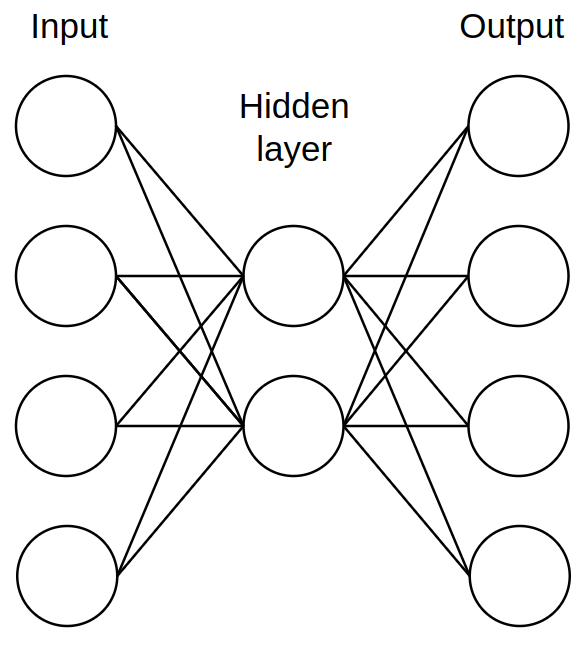
\includegraphics[width=0.6\textwidth]{figures/2_/2_undercomplete_autoencoder.png}
        \caption{An undercomplete autoencoder: the dimension of the smallest hidden layer is less than the input dimension.}
        \label{fig:2_undercomplete_autoencoder}
    \end{subfigure}
    \hfill
    \begin{subfigure}[b]{0.45\textwidth}
        \centering
        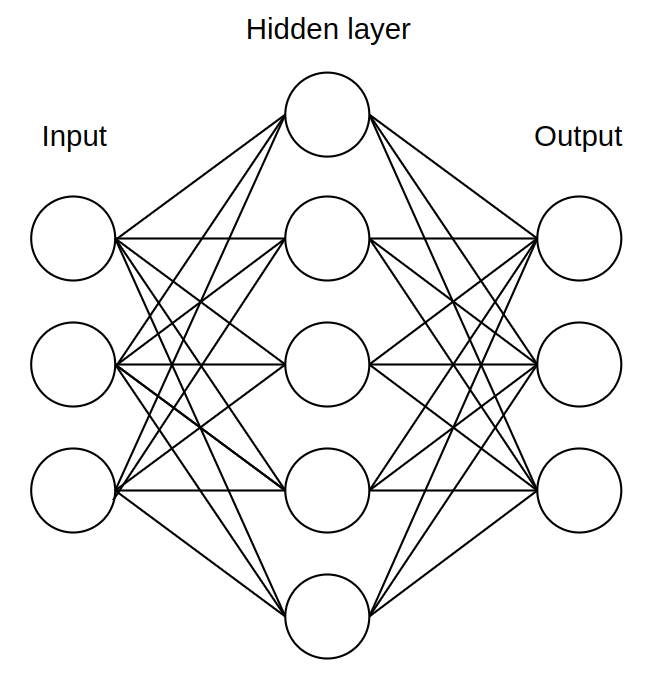
\includegraphics[width=0.8\textwidth]{figures/2_/2_overcomplete_autoencoder.png}
        \caption{For comparison, a sparse autoencoder has sufficient hidden units but has a sparsity constraint imposed on its hidden layer.}
        \label{fig:2_overcomplete_autoencoder}
    \end{subfigure}
    \caption{The difference between an undercomplete and sparse autoencoder.}
    \label{fig:2_autoencoders}
\end{figure}
As a result, undercomplete autoencoders are forced to capture the most prominent features of the input data in its hidden layer \cite{DeepLearningBook}. 

To train an undercomplete autoencoder, we minimise a loss function,
\begin{equation}
    \loss\,(\bx, \, g(f(\bx)))
\end{equation}
where we set the target values of the neural network to be equal to the input $\bx$. The loss function is normally chosen to be the mean-squared error (MSE) between the input and the reconstructed input,
\begin{equation}
    \loss_{MSE} = \sum_{x_i \in \bx} \big[x_i - g(f(x_i))\big]^2 \label{eq:2_autoencoder_mse}
\end{equation}
and the neural network is optimised through a standard optimisation algorithm, such as mini-batch stochastic gradient descent.
The loss can also be chosen as the binary cross-entropy between input and reconstruction depending on the task, for example, when encoding Bernoulli distributed data or one-hot encoded text.
For the sake of completeness, a sparse autoencoder has almost the same objective, but with an added penalty term $\Omega(\bz)$ (e.g. L1 loss) that enforces sparsity (keep weights close to 0) in the hidden layer $\bz$ \cite{DeepLearningUnipdItaly}.


\subsection{Variational Autoencoders}
\label{subsec:2_VAE_variational_autoencoders}

Variational autoencoders (VAEs) \cite{variational_bayes, vae_stochastic_backprop} are related to autoencoders in terms of architecture, but are in the family of \textit{structured probabilistic models}. This means that they also have an encoder-decoder neural network structure but, in contrast, make assumptions on the underlying probability distribution of the input $\bx$ and latent code $\bz$ and wish to model it.

\subsubsection{A Parametrised Probabilistic Model}
\begin{figure}[H]
    \centering
    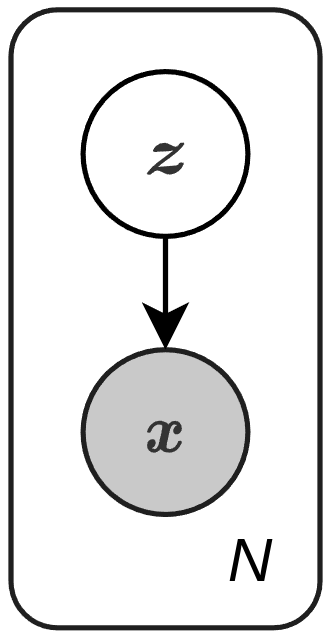
\includegraphics[width=0.15\textwidth]{figures/2_/2_general_vae.png}
    \caption{A graphical model (Bayes net) of the probability model in the VAE. The assumption is that our observed input data $\bx$ is generated from the conditional distribution $\pbts(\bx|\, \bz)$, with true parameters $\bt^*$ unknown. Here, the latent representation $\bz$ is hidden, while the input $\bx$ is observed (grey). $N$ is the number of repetitions (in plate notation), equivalent to the number of i.i.d. samples of some dataset.}
    \label{fig:2_general_vae}
\end{figure}
VAEs contain a probabilistic model, with parameters $\bt$, that aims to estimate a joint probability distribution $\pbts(\bx, \bz)$ as shown in \cref{fig:2_general_vae}.  It assumes that our latent variables $\bz$ are generated from some prior distribution $\pbts(\bz)$ and that the input $\bx$ is generated from the conditional distribution $\pbts(\bx|\, \bz)$. Also, it is assumed that the prior $\pbts(\bz)$ and likelihood $\pbts(\bx|\, \bz)$ both come from parametric families of distributions $\pbt(\bz)$ and $\pbt(\bx|\, \bz)$, though their true parameters $\bt^*$ are unknown \cite{variational_bayes}.

The main use of learning this joint distribution is so that the probabilistic model can perform \textit{probabilistic inference} -- computing the posterior distribution of the hidden nodes, given the values of observed nodes \cite{murphy2012machinelearningBook}:
\begin{equation}
    \pbt(\bz |\, \bx) = \frac{\pbt(\bx |\, \bz) \pbt(\bz)}{\pbt(\bx)}
\end{equation}
From a representation learning perspective, being able to learn how to perform posterior inference requires that a probabilistic model learns the distribution of the data $\pbt(\bx)$, which then allows the model to infer the hidden structure or latent code $\bz$ that best explains our input $\bx$ \cite{stochastic_variational_inference}.

However, exact inference is often intractable due to $\pbt(\bx) = \int \pbt(\bz) \, \pbt(\bx |\, \bz)$ requiring a marginalisation of over the latent variables (which is exponential in the number of hidden nodes) and because of the scale of large datasets \cite{variational_bayes}. Therefore, VAEs instead make use of \textit{variational inference}: attempting to approximate the true posterior $\pbt(\bz |\, \bx)$ with a restricted family of distributions $\qbp(\bz |\, \bx)$, where the goal is to find the settings of the variational parameter $\boldsymbol{\phi}$ that best approximates the true posterior. This transforms a complex inference problem into a high-dimensional optimisation problem \cite{stochastic_variational_inference, DeepLearningBook}.

So, in machine learning terms, the encoder neural network of a VAE parametrised by $\boldsymbol{\phi}$ represents the approximate posterior $\qbp(\bz |\, \bx)$, and generates a family of distributions -- such as a set of means and variances for Gaussians -- for a given datapoint $\bx$. Similarly, the decoder neural network, parametrised by $\boldsymbol{\theta}$, then represents the corresponding likelihood distribution $\pbt(\bx |\, \bz)$ that generates a distribution over values of $\bx$ for a given latent code $\bz$. 
In the literature, the probabilistic encoder is also referred to as an \textit{inference network} or \textit{recognition model}, while the probabilistic decoder is referred to as a \textit{generative network} or \textit{generative model}.

\subsubsection{Optimising the VAE}
Now, in order to optimise the parameters of the encoder and decode, we want to find an objective function to update parameters $\boldsymbol{\phi}$ and $\boldsymbol{\theta}$ so that our encoder $\qzgivex$ best approximates the true posterior $\pzgivex$, and that our generative decoder $\pbt(\bx |\, \bz)$ best approximates the true likelihood $\pbts(\bx|\, \bz)$. To do this, we first have to consider a non-negative similarity measure, the \textit{Kullback-Leibler (KL) divergence}, that can be used to measure the difference between two distributions $P(x)$ and $Q(x)$ \cite{DeepLearningBook}:
\begin{equation}
    \DKL{P}{Q} = \E_{x \sim P} \left[ 
    \log \frac{P(x)}{Q(x)}
    \right] =
    \E_{x \sim P} \left[ 
    \log P(x) - \log Q(x)
    \right]
\end{equation}
Then, with the goal of minimising the difference between the approximate $\qzgivex$ and true posterior $\pzgivex$, we can substitute these for $P(x)$ and $Q(x)$ to get:
\begin{align*}
    \DKL{\qzgivex}{\pzgivex} 
    =& \Ewrtq \left[ 
    \log \qzgivex - \log \pzgivex
    \right] \\
    =& \Ewrtq \left[ 
    \log \qzgivex - \log \frac{\pbt(\bx ,\, \bz)}{\pbt(\bx)}
    \right] \\
    =& \Ewrtq \left[\log \qzgivex \right] - \Ewrtq \big[ \log \pbt(\bx ,\, \bz)
    \big] + \log \pbt(\bx) \numberthis
\end{align*}
However, this term cannot be computed directly due to the marginal likelihood $\pbt(\bx)$ being intractable as mentioned above. To get around this, we instead rewrite the marginal likelihood as:
\begin{equation}
    \log \pbt(\bx) = \DKL{\qzgivex}{\pzgivex} +
    \loss \,(\boldsymbol{\theta}, \boldsymbol{\phi}; \bx)
\end{equation}
Since the KL divergence is non-negative, the term $\loss\,(\boldsymbol{\theta}, \boldsymbol{\phi}; \bx)$ is referred to as the \textit{variational lower bound} or \textit{evidence lower bound (ELBO)} since it sets a lower bound on the marginal likelihood (or evidence) \cite{variational_bayes}:
\begin{equation}
    \log \pbt(\bx) \geq \loss\,(\boldsymbol{\theta}, \boldsymbol{\phi}; \bx) = \Ewrtq \left[-\log \qzgivex + \log \pbt(\bx ,\, \bz)
    \right]
\end{equation}
This can be rewritten further:
\begin{align*}
    \loss\,(\boldsymbol{\theta}, \boldsymbol{\phi}; \bx) =& 
    \Ewrtq \left[-\log \qzgivex 
    + \log \pbt (\bx |\, \bz)
    + \log \pbt (\bz)
    \right] \\
    =& - \Ewrtq \left[\log \qzgivex 
    - \log \pbt (\bz)
    \right]
    +  \Ewrtq \big[ \log \pbt (\bx |\, \bz) \big] \\
    =& -\DKL{\qzgivex}{\log \pbt(\bz)}
    +  \Ewrtq \big[ \log \pbt (\bx |\, \bz) \big] \numberthis
    \label{eq:2_vae_loss}
\end{align*}

This ELBO term is particularly interesting because \textit{maximising} it is equivalent to \textit{minimising} the KL divergence between the approximate and true posteriors. Therefore, we choose to optimise this term through a standard optimisation algorithm, such as mini-batch stochastic gradient \textit{ascent}. For a single datapoint with $L$ samples, an estimator for the ELBO loss in \eqref{eq:2_vae_loss} is:
\begin{equation}
    \widetilde{\loss}\,(\boldsymbol{\theta}, \boldsymbol{\phi}; \bx^{(i)}) = 
    -
    \DKL{\qbp(\bz |\, \bx^{(i)})}{\log \pbt(\bz)}
    +   
    \frac{1}{L} \sum^{L}_{l=1} \big(
    \log \pbt (\bx^{(i)} |\, \bz^{(i,l)}) 
    \big)
    \label{eq:2_vae_loss_estimator_single_datapoint}
\end{equation}
This can be extended to be an estimator for the ELBO loss for the full dataset:
\begin{equation}
    \loss\,(\boldsymbol{\theta}, \boldsymbol{\phi}; \bx^{(i)}) 
    \simeq
    \widetilde{\loss}^M\,(\boldsymbol{\theta}, \boldsymbol{\phi}; \bx^{(i)}) 
    =
    \frac{N}{M} \sum^{M}_{i=1} \left(
    \widetilde{\loss}\,(\boldsymbol{\theta}, \boldsymbol{\phi}; \bx^{(i)})
    \right)    \label{eq:2_vae_loss_estimator_dataset}
\end{equation}
where $M$ is the number of datapoints per mini-batch and $N$ the total datapoints. By choosing $M$ large enough (e.g. $M=100$) allows us to use have one sample per datapoint ($L=1$) when computing \eqref{eq:2_vae_loss_estimator_single_datapoint} \cite{variational_bayes}. We also note for later reference that the first term in \eqref{eq:2_vae_loss_estimator_single_datapoint} can be referred to as a \textit{regularisation loss}, while the second term can be referred to as a \textit{reconstruction loss}.

\subsubsection{The Reparametrisation Trick}
However, since $\bz$ is a random variable sampled from the distribution $\qzgivex$, how are we able to find \textit{deterministic} gradients of the ELBO with respect to the parameters $\boldsymbol{\phi}$ of the distribution $\qzgivex$? 
To solve this, \cite{variational_bayes} introduced a \textit{reparametrisation trick} where, for a datapoint $\bx^{(i)}$, the continuous \textit{random} variable $\bz^{(i,l)} \sim \qbp(\bz |\, \bx^{(i)})$
 is expressed as a \textit{deterministic} variable:
\begin{equation}
    \bz^{(i,l)} = 
    \gbp(\boldsymbol{\epsilon}^{(i,l)}, \bx^{(i)}), \qquad \text{where} \qquad
    \boldsymbol{\epsilon}^{(l)} \sim p(\boldsymbol{\epsilon})
\end{equation}
and $\boldsymbol{\epsilon}$ being a noise variable  with marginal distribution $p(\boldsymbol{\epsilon})$.
By reparametrising $\bz$ through a differentiable transformation $\gbp(\boldsymbol{\epsilon}^{(i,l)}, \bx^{(i)})$ and $\boldsymbol{\epsilon}$, we ensure that the parameters of the distribution still remain learnable while the VAE remains stochastic through $\boldsymbol{\epsilon}$. To give an example, in most cases, we assume the variational approximate and true posteriors to be a multivariate Gaussian. To sample $\bz^{(i,l)}$ using the reparametrisation trick would be done as:
\begin{equation}
    \bz^{(i,l)} = 
    \boldsymbol{\mu}^{(i)} + \boldsymbol{\sigma}^{(i)} \odot \boldsymbol{\epsilon}^{(l)},
    \qquad \text{and} \qquad
    \boldsymbol{\epsilon}^{(l)} \sim \mathcal{N}(\boldsymbol{0}, \textbf{I})
\end{equation}
with $\odot$ meaning the element-wise product.
In this example, the mean $\boldsymbol{\mu}^{(i)}$ and standard deviation $\boldsymbol{\sigma}^{(i)}$ of the Gaussian would then become learnable parameters of the encoder, each having their own deterministic gradients that can be calculated in backpropagation.

\subsubsection{Understanding ELBO and the VAE Latent Space}
Finally, using a VAE gives the learned latent representation $\bz$, for a given input $\bx$, some desirable properties that distinguish it from ordinary autoencoders.

First, by observing the structure of \eqref{eq:2_vae_loss_estimator_single_datapoint}, we note that to maximise the ELBO loss requires that we minimise the KL divergence between the approximate posterior $\qzgivex$ and the latent prior $\pbt(\bz)$. When we assume both to be multivariate Gaussians, $\qzgivex$ is essentially penalised for being ``different'' from a Gaussian distribution.
Then, by forcing the approximate posterior distribution to be similar to some pre-decided prior distribution $\pbt(\bz)$, we can sample $\bz$ from this prior and generate synthetic data through the decoder $\pxgivez$. To visualise how the latent space influences the generated data, we can also perform a systematic sampling of the latent space, such as in a $[-1, 1]$ area for a Gaussian two-dimensional latent space, to generate a manifold (or prior predictive distribution) as shown in \cref{fig:2_manifolds}.
\begin{figure}[hbt]
    \begin{subfigure}[b]{0.41\textwidth}
        \centering
        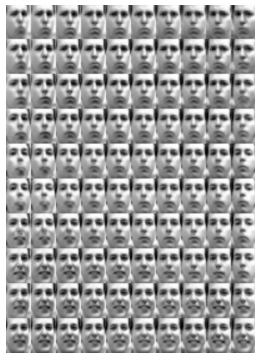
\includegraphics[width=0.7\textwidth]{figures/2_/2_face_manifold.png}
        \caption{Learned Frey Face manifold}
        \label{fig:2_face_manifold}
    \end{subfigure}
    \hfill
    \begin{subfigure}[b]{0.57\textwidth}
        \centering
        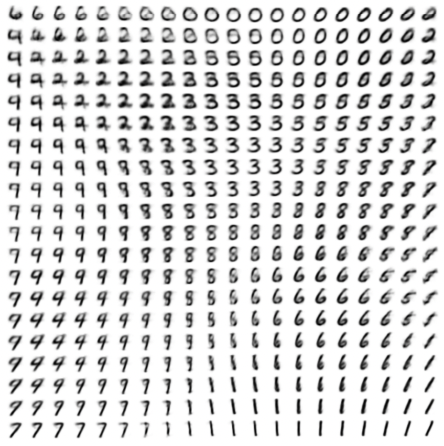
\includegraphics[width=0.7\textwidth]{figures/2_/2_mnist_manifold.png}
        \caption{Learned MNIST manifold}
        \label{fig:2_mnist_manifold}
    \end{subfigure}
    \caption{The predicted manifolds generated from sampling latent variables $\bz$ in a linearly spaced $[-1, 1]$ area when $\pbt(\bz)$ is 2D Gaussian. Both images are obtained from \cite{variational_bayes}.}
    \label{fig:2_manifolds}
\end{figure}
Therefore, by placing the prior assumption on the underlying distribution of our approximate posterior and latent space distribution, VAEs are capable of being \textit{generative models}. 

To understand the ELBO loss further, \cite{variational_bayes} refers to the first KL divergence term in \eqref{eq:2_vae_loss_estimator_single_datapoint} as a \textit{regulariser}, while the second term can be thought of as a \textit{reconstruction error}. Looking first at the reconstruction term, we recall that the objective of most machine learning models is that of maximum likelihood estimation (MLE) (minimising the negative log-likelihood might sound familiar). The goal of MLE is to find the parameters of a model that maximises the likelihood that they generated the data -- or, in this case, finding the best $\boldsymbol{\theta}$ so that $\pxgivez$ most accurately describes the process that generated our data, which was assumed to be the unknown likelihood distribution $\pbts(\bx |\, \bz)$. So, by maximising the log-likelihood in \eqref{eq:2_vae_loss_estimator_single_datapoint}, we are doing MLE, which is equivalent to finding the best model parameters that minimises the reconstruction error between a target -- the input generated from $\pbts(\bx |\, \bz)$ -- and output generated from our decoder $\pbt(\bx |\, \bz)$.

Next, the KL divergence term can be considered a regulariser by first remembering that it penalises the encoder for being ``different'' from a Gaussian prior. 
Further, given that it is not entirely likely that the true unknown posterior $\pbts(\bz |\, \bx)$ follows a Gaussian distribution, it will be natural to incur an information loss (and so a high KL divergence) when we assume that our approximate posterior is.
Therefore, there is a trade-off between learning a proper input reconstruction (when the approximate posterior deviates from a Gaussian) versus staying close to the Gaussian prior. This constraint can be thought of as limiting the generative capacity of the VAE when compared to having no KL divergence loss in the ELBO, but its regulatory effect places emphasis on the VAE having to learn \textit{meaningful and statistically independent latent factors} \cite{betaVAEHiggins2017}. In other words, it is expensive for the latent variables to deviate from the Gaussian prior, so the latent variables that do deviate should hold meaningful and independent information -- i.e. they each describe their own features of the input -- so that a reduction in the reconstruction error compensates for their incurred cost.

To summarise, the goal of VAEs is to minimise the KL divergence between the true and approximate variational posteriors, $\DKL{\qzgivex}{\pzgivex}$. 
This was intractable due to the marginal likelihood $\pbt(\bz)$, and so it was shown that this was equivalent to maximising the ELBO loss in \eqref{eq:2_vae_loss_estimator_single_datapoint}. The effect of formulating the objective function in this way had two consequences. Firstly, the VAE achieved a desirable, well-formed latent space (most often close to a Gaussian prior). This allowed VAEs to be generative since, to generate ``synthetic'' data, we could sample latent variables following the prior distribution and compute $\pxgivez$. Second, the KL divergence term served as a regulariser which motivated latent variables in the VAE to hold meaningful representations of the input distribution.

\subsection{Convolutional Variational Autoencoders}
\label{subsec:2_conv_VAEs}
Convolutional variational autoencoders are VAEs that utilise \textit{convolutional neural networks} (CNNs) to parametrise the encoder and some \textit{deep generative deconvolutional network} (DGDN) to parametrise the decoder \cite{conv_vae}. The theory behind this is that for structured data, convolutional operations are best suited for feature extraction, being ``tremendously successful'' in practice \cite{DeepLearningBook}. Therefore, when tasked with learning an unsupervised representation of (for example) images, we can use these instead of fully-connected VAEs.

\subsubsection{Convolution}
CNNs are simply NNs that use the convolution operation ($*$) instead of general matrix multiplication in at least one of their layers \cite{DeepLearningBook}. If we consider a function $x(t)$, convolutions can be understood as a an operation $(w*x)$ that describes how one function $x(t)$ is affected by a second function $w(t)$. Intuitively, we can think of $x(t)$ as our input and $w(t)$ as some weighting for our input $x(t)$, where the weights $w(t)$ are the weights of our neural network.
Explicitly, convolution for one-dimensional inputs where both functions are a function of time $t$, produces a function $s$ \cite{DeepLearningBook}:
\begin{equation}
    s(t) = (x * w)\,(t) = \sum^\infty_{a=-\infty} x(a)\, w(t-a)
\end{equation}
Note that if $w(t)$ is a weighted average function, convolution resembles \textit{Bayesian smoothing}.

Convolutions can also be extended to two-dimensional inputs. In this case, we normally refer to the first argument as input $I$, and the second as a \textit{filter} or \textit{kernel} $K$. This gives a \textit{feature map} $S$:
\begin{equation}
S\,(i, j) = (I * K)\,(i, j) = \sum_{m}\sum_{n} I(m, n) \, K(i - m, j - n) \label{eq:2_2d_convolution}
\end{equation}
Though in practice, we actually use \textit{cross-correlation} to represent convolution \cite{DeepLearningBook}:
\begin{equation}
S\,(i, j) = (K * I)\,(i, j) = \sum_{m}\sum_{n} I(i + m, j + n) \, K(m, n) \label{eq:2_2d_convolution_cross_correlation}
\end{equation}
This operation is perhaps most familiar to us, where we recognise that for a kernal $K$ of size $m\times n$, the output at index $(i,j)$ is given by a simple matrix multiplication of the kernal with a specific region of the input. This is also how \cite{RectifiersKaimingHe2015} represents convolution:
\begin{equation}
    \boldsymbol{y}_l = \boldsymbol{W}\boldsymbol{x}_l + \boldsymbol{b}_l
\end{equation}
where $\boldsymbol{x}$ is an $m\times n$-by-1 vector that represents co-located $m \times n$ pixels, and $\boldsymbol{W}_l$ is a $d$-by-$m\times n$ matrix where $d$ represents the number of kernels for convolution.

\subsubsection{Deconvolution}
Mathematically, deconvolution is defined as the inverse of convolution. However in the literature, deconvolution is also used to describe a series of \textit{convolution-unpooling (convolution-upsampling)} operations \cite{conv_vae} or \textit{transposed convolutions}\footnote{The authors of \cite{deconv_visualised} provide a very tidy visualisation of transposed convolutions at: \url{https://github.com/vdumoulin/conv_arithmetic}}.
For the purpose of this thesis, we focus on the use of transposed convolutions to represent deconvolution.

Transposed convolutions are designed by swapping the forward and backward passes of a convolution. As mentioned, the forward pass of a convolution operation can be expressed as the matrix multiplication of a set of co-located pixels $\boldsymbol{x}_l$ with a kernel $\boldsymbol{W}_l$. When calculating the gradient of $\boldsymbol{y}_l$ w.r.t. the kernel $\boldsymbol{W}_l$ in backpropagation, this becomes instead a multiplication of the feature map $\boldsymbol{y}_l$ with the transposed kernel $\boldsymbol{W}^\top_l$. So, in another sense, transposed convolutions can be thought of as a function applied on a feature map such that its output is the initial input used to create the initial feature map \cite{deconv_visualised}. 
Therefore, transposed convolution layers make use of this idea as a sort of pseudo-inverse of convolution and allows it to also recover the shape of the input. 

\subsubsection{The Encoder and Decoder of a Convolutional VAE}
As mentioned earlier, convolutional VAEs are comprised of a CNN as an encoder and some deconvolution network that serves as the decoder. Here, the CNN uses the convolution operation in place of a full matrix multiplication, while the deconvolution network applies transposed convolutions as a pseudo-inverse to the convolution operation.
Apart from this technical distinction, convolutional VAEs are optimised in exactly the same way as fully-connected ones -- using the loss specified in \eqref{eq:2_vae_loss_estimator_single_datapoint} and \eqref{eq:2_vae_loss_estimator_dataset} -- such that the CNN parametrises the approximate posterior distribution $\qzgivex$, while the deconvolution network parametrises the likelihood distribution $\pxgivez$. 


\subsection{A Practical Note on the VAE Reconstruction Loss}
\label{subsec:2_vae_recons_loss}
When implementing the VAE loss function \eqref{eq:2_vae_loss_estimator_single_datapoint}, we can represent the reconstruction loss either through the \textit{binary cross-entropy (BCE)} or \textit{mean-squared error (MSE)}, though these are not entirely equivalent.
The reason for this is that both loss functions are actually founded in MLE and minimising them is also equivalent to minimising the negative log-likelihood of our data $p_{\text{data}}(\bx)$ given our model $p_{\bt}(\bx)$ \cite{DeepLearningBook}. The main difference for their use lies in the what we assume the distribution of our data $p_{\text{data}}(\bx)$ to be, as this assumption lays the ground for how we optimise for $\bt$.
To see how we can extend the theory from Section 5.5 of \cite{DeepLearningBook} to two fundamental examples.

Essentially, in MLE we define the conditional maximum likelihood estimator $\bt$ for predicting observed targets $\boldsymbol{y}^{(i)}$ from samples $\bx^{(i)}$ to be:
\begin{equation}
    \bt_{\text{ML}} = \argmax_{\bt} \sum^m_{i=1} \log p_{\bt}(\boldsymbol{y}^{(i)} \,|\, \bx^{(i)}) 
    \label{eq:2_ml_loss}
\end{equation}
where $m$ is the number of samples available. When assuming $p_{\text{data}}(\boldsymbol{y}^{(i)} \,|\, \boldsymbol{x}^{(i)})$ follows a Gaussian distribution $\mathcal{N}(\boldsymbol{y}; \hat{\boldsymbol{y}}^{(i)}, \sigma)$, where $\hat{\boldsymbol{y}}^{(i)}$ is the predicted mean for a Gaussian distributed $\bx^{(i)}$ (with fixed $\sigma$ for simplicity), we can rewrite the log-likelihood based on the well-known Gaussian probability distribution function (PDF):
\begin{equation}
    \sum^m_{i=1} \log p_{\bt}(\boldsymbol{y}^{(i)} \,|\, \bx^{(i)}) = m \log \sigma - \frac{m}{2} \log (2\pi) - \sum^m_{i=1} \frac{||\hat{\boldsymbol{y}}^{(i)} - \boldsymbol{y}^{(i)}||}{2 \sigma^2}
\end{equation}
From this we can identify the similarity with the MSE loss:
\begin{equation}
    \loss_{\text{MSE}} = \frac{1}{m} \sum^m_{i=1} \frac{||\hat{\boldsymbol{y}}^{(i)} - \boldsymbol{y}^{(i)}||}{2 \sigma^2}
    \label{eq:2_mse_loss}
\end{equation}

Alternatively, if we assume that our data-generating distribution $p_{\text{data}}(\boldsymbol{y}^{(i)} \,|\, \boldsymbol{x}^{(i)})$ follows a Bernoulli distribution $\text{Ber}(\boldsymbol{y}^{(i)}; \hat{p}^{(i)})$, with $\boldsymbol{y}^{(i)} \in \{0, 1\}$ as the observed class and $\hat{p}^{(i)} \in (0, 1)$ as the predicted probability of $\boldsymbol{y}^{(i)}$ in class 1, its less-known probability mass function (PMF) is given by:
\begin{equation}
    p_{\bt}(\boldsymbol{y}^{(i)} \,|\, \boldsymbol{x}^{(i)}) = \hat{p}^{{(i)}^{\boldsymbol{y}^{(i)}}}
    (1 - \hat{p}^{{(i)}^{1 - \boldsymbol{y}^{(i)}})}
\end{equation}
Then, we can rewrite the maximum likelihood objective in \eqref{eq:2_ml_loss} using this:
\begin{align}
    \sum^m_{i=1} \log p_{\bt}(\bx^{(i)}) &=  \sum^m_{i=1} \log \bigg(\hat{p}^{{(i)}^{\boldsymbol{y}^{(i)}}} \Big(1 - \hat{p}^{{(i)}^{1 - \boldsymbol{y}^{(i)}}} \Big)\bigg) \\
    &=  \sum^m_{i=1} \boldsymbol{y}^{(i)} \,\log \,\hat{p}^{(i)} +  (1 - \boldsymbol{y}^{(i)}) \log (1 - \hat{p}^{(i)})
\end{align}
From which we identify the BCE loss:
\begin{equation}
    \loss_{\text{BCE}} = \frac{1}{m} \sum^m_{i=1} \boldsymbol{y}^{(i)} \log \hat{p}^{(i)} +  (1 - \boldsymbol{y}^{(i)}) \log (1 - \hat{p}^{(i)})
\end{equation}

So from these examples, we see that \textit{BCE} is generally used when we assume our data is \textit{Bernoulli distributed}, e.g. a (black-white) pixel value is either 0 or 1, while \textit{MSE} is used when we assume that our data is \textit{Gaussian distributed}, e.g. the heights of students in Trondheim.

To apply this to VAEs, since we wish to optimise the parameters of our generative network $\bt$ to reconstruct our input $\bx^{(i)}$, we replace the observed targets $\boldsymbol{y}^{(i)}$ with our input $\bx^{(i)}$, while the reconstructions $\br^{(i)} \sim \pxgivez$
serve as the model prediction $\hat{\bx}^{(i)}$. The choice for the loss function, however, is unclear. Whether one chooses to assume that the data-generating distribution $\pbts(\bx|\, \bz)$ with unknown parameters $\bt^*$ is best approximated through a family of Gaussians or family of Bernoulli distributions is left as a design choice, as we have no indication of the true shape of its distribution.
Though as consolidation, the optimal parameters $\bt$ for our model $\pxgivez$ are the same no matter which loss function is used, only the loss values are different \cite{DeepLearningBook}. 

\section{Reinforcement Learning}
\label{sec:2_RL}
Reinforcement learning is a learning-based method for discovering complex behaviour without explicit programming. It allows an agent to capture the dynamics of a system and the uncertainties of the environment through a data-driven approach, using a high-abstraction, evaluative feedback or \textit{reward} \cite{RLinRoboticsSurvey}.

To get an overview of the basics of reinforcement learning, we can begin by looking into its definition and goal. Sutton and Barto \cite{suttonAndBartoBook} states, “reinforcement learning is learning what to do – how to map situations to actions – so as to maximise a numerical reward signal.” Further, \cite{RLinRoboticsSurvey} adds, “reinforcement learning enables a robot to autonomously discover an optimal behaviour through trial-and-error interactions with its environment." 
From these, there are many terms that could be examined, such as, \textit{situations}, \textit{actions}, \textit{rewards}, \textit{behaviour}, \textit{trial-and-error interactions} and \textit{environment}. We can ask ourselves, “what exactly is an optimal behaviour and how to we express this?”.
Throughout this section, we will cover these central concepts, where in the end, we will explore how \textit{temporal-difference learning}, \textit{actor-critics} and \textit{proximal policy optimisation} algorithms enable us to discover an optimal behaviour.

As reinforcement learning was the central theme of the project thesis, much of the fundamental theory in the following sections is shared with that in the project \cite{project_thesis}. As a result, many of the following subsections are taken from the project thesis, being only partially rewritten and marked with an asterisk (*).

\subsection{Finite Markov Decision Processes*}
\label{subsec:2_MDPs}

Finite Markov Decision Processes (MDPs) are a way of formalising how an agent interacts with the environment, serving as a standardised learning framework for reinforcement learning. MDPs are often depicted as an iterative diagram as shown in \cref{fig:2_MDP}, comprising of five elements: the \textit{agent}, \textit{environment}, \textit{state} $S_t$, \textit{action} $A_t$ and \textit{reward} $R_t$.
\begin{figure}[hbt]
    \centering
    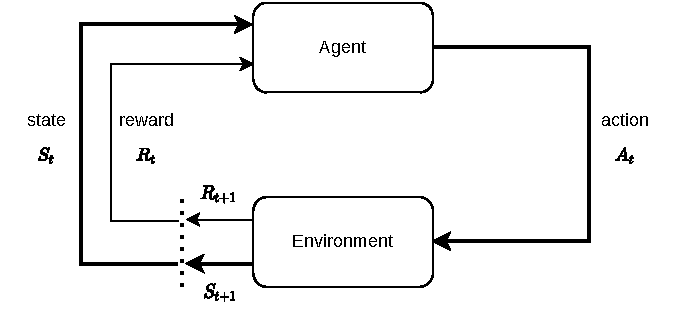
\includegraphics[width=0.7\textwidth]{figures/2_RL/2_mdp.pdf}
    \caption{The interaction between agent and environment in an MDP, from \cite{suttonAndBartoBook}.}
    \label{fig:2_MDP}
\end{figure}
MDPs are an extension of stochastic Markov chains, where state transitions from $S_t$ to $S_{t+1}$ are now influenced by a choice in action $A_t$, and each transition also yields a reward $R_t$.

To go into detail, an \textit{agent} has a task of \textit{learning} how to solve a specific task, whereby improving its performance through \textit{experience} -- simply a set of repeated state-action interactions with the environment. 
The \textit{environment} contains the task to be solved and essentially everything an agent interacts with, for example, the system dynamics and the rewards for being in certain states. From a cybernetics perspective, the agent serves as a controller while the environment can be understood as the plant or process to be controlled.
The situations that an agent finds itself in is referred to as \textit{states} or \textit{observations}. Each of the states in an MDP also has the Markov Property, which means that all the information in state $S_t$ is only dependent on the previous state $S_{t-1}$ and action $A_{t-1}$. 
For any state $S_t \in \mathcal{S}$, the agent can take an \textit{action} $A_t \in \mathcal{A}(s)$, where $\mathcal{S}$ represents the state-space or set of possible states and $\mathcal{A}(s)$ the action-space or set of possible actions for $S_t$. Actions generally refer to anything that transitions an agent into a new state and may vary largely from task to task. An example of this could be a control signal from a controller, such as the torques for each rotor on a quadrotor, though it could also be reference signals from an optimal controller, such as velocity references for a controller to follow.

Moreover, the states that an agent finds itself is determined by the \textit{initial state distribution} $p(s)$, while the states the agent moves to follows the \textit{state-transition distribution} $p(s',\, r\, |\, s,\, a)$. The state-transition distribution is a function of four arguments that captures the dynamics of the MDP and describes the probability of a specific transition within the environment \cite{suttonAndBartoBook}:
\begin{equation}
    p(s',\, r\, |\, s,\, a) = P(S_t = s',\, R_t = r\, |\, S_{t-1} = s,\, A_{t-1} = a)
\end{equation}
Here, $S_t$, $R_t$ and $A_t$ are random variables with well-defined probability distributions while the lower case letters $s$, $r$ and $a$ refer to specific values of these variables. The value $s'$ is commonly used to denote the value of the next state from $s$.

Lastly, we see that for each state transition an agent receives a numerical \textit{reward} $R_t \in \mathcal{R} \subset \mathbb{R}$, which can be interpreted as an evaluative feedback for a choice of action $A_t$. The reward is commonly a function of the current state and action values, $R(s, a)$, and is often the main tool used to shape agent behaviour in the environment \cite{RLinRoboticsSurvey}. 

Finally, the MDP can be modelled as a tuple ... \todo{Can be defined by a tuple S, A, transition dynamics, r, p0, gamma}


\subsection{Returns*}
\label{subsec:2_returns}

Now that we have formalised agent-environment interactions, we can imagine that by trying enough actions in different states, the agent will discover an optimal behaviour - essentially choosing the ``best'' action for every possible state $S_t \in \mathcal{S}$. Yet, what exactly is the ``best'' action for each state $S_t$? Is it the state-action pair with the highest reward $R_t$? 

To answer this, we can start by defining the goal of reinforcement learning. As mentioned at the beginning of the section, reinforcement learning aims to, informally, “maximise a numerical reward signal”. The reward signal, in this case, is a scalar received every time step at each new state and serves as an immediate feedback for the agent's action. Yet, if we consider the formulation of MDPs more carefully, taking a certain action in a particular state does not only affect the state the agent transitions to in the next time step, but also all consequent states and rewards for all following time steps. This illustrates the concept of \textit{delayed reward}, which suggests that receiving a high reward now does not necessarily mean receiving a high reward later.

Therefore, it is important to define the goal of reinforcement learning in the context of reward more precisely. As such, the return $G_t$ is defined as a function of a specific sequence of rewards, $R_{t+1}$, $R_{t+2}$, $R_{t+3}$ .... For example, the simplest return can be defined as the sum of the reward sequence \cite{suttonAndBartoBook}:
\begin{equation}
    G_t = R_{t+1} + R_{t+2} + ... + R_{T}
\end{equation}
With this, we generally seek to maximise the \textit{expected} return over some time horizon:
\begin{equation}
    J = \E \, [G_t] = \E \, \left[ 
    \sum^{T}_{k = t+1} R_k
    \right]
\end{equation}
Here, $T$ represents the time of termination and is a random variable that normally varies with each \textit{episode}. An episode in this case refers to a sequence of timesteps for which an agent is performing a task until the agent reaches a \textit{terminal state}. 

However, in control tasks, we see that there is often no defined terminal state but rather an indefinite continuing process, such as in process control. Therefore, it is common to instead maximise the \textit{discounted return} \cite{suttonAndBartoBook}:
\begin{equation}
    J = \E \, [G_t] = \E \, \left[ 
    \sum^{T}_{k = 0} \gamma^{k} R_{k+t+1}
    \right]
\end{equation}
where $\gamma^k \in [0, 1)$ is referred to as the \textit{discount factor} -- an exponentially decreasing weight on \textit{future rewards}, often chosen to be 0.99. The discount factor ensures that for any timestep $t$ the infinite sum of rewards is finite, allowing the agent to evaluate returns that are defined for each time step.
Another interesting property that should be noted -- and will be important for concepts later -- is the recursive expression for the return $G_t$:
\begin{align}
    G_t &= R_{t+1} + \gamma R_{t+2} + \gamma^2 R_{t+3} + \gamma^3 R_{t+4} ... \nonumber \\
    G_t &= R_{t+1} + \gamma (R_{t+2} + \gamma R_{t+3} + \gamma^2 R_{t+4} ...) \nonumber \\
    G_t &= R_{t+1} + \gamma G_{t+1} \label{eq:2_recursive_returns} 
\end{align}

So, with the goal of reinforcement learning defined more clearly in terms of maximising the expected discounted return, we now need to have a formal definition for the agent behaviour before we can optimise it.

\subsection{Policies and Value Functions*}
\label{subsec:2_policies_and_value_funcs}

First, the behaviour that an agent learns is referred to as a policy $\pi$. Policies define a mapping of states to probabilities of selecting each possible action, $\pi(s \,|\, a) = P(a\,|\,s)$ \cite{suttonAndBartoBook}. Despite this, a policy $\pi$ can also be deterministic, resulting in the same action for a state every time, written as $a = \pi(s)$ \cite{RLinRoboticsSurvey}.


Initially, we can imagine that policies are quite random and non-idea. Then throughout the learning process, the agent will receive rewards $R_t$, accumulate returns $G_t$, and update its policy $\pi$ consequently. So, when we think about an optimal policy $\pi^*$, we imagine an agent performing the actions that result in the best result.
Hence, we can say that in order to solve the reinforcement learning problem, we need to ``solve'' the MDP by finding this optimal policy $\pi^*$.

The method forward is to define a \textit{state-value function} $V^\pi$, which indirectly tells us how good it is to be in a particular state. For MDPs, the state-value function can be defined as the expected return for being in a state $s$ and following a policy $\pi$ thereafter \cite{suttonAndBartoBook}:
\begin{equation}
    V^\pi(s) = \E_\pi [G_t \hspace{0.5mm} | \hspace{0.5mm} S_t = s] = \E_\pi \left[\sum^\infty_{k=0} \gamma^t R_{t+k+1} \hspace{0.5mm} \Bigg| \hspace{0.5mm} S_t = s \right] \forall s \in \mathcal{S}
\end{equation}
Similarly, we can define an \textit{action-value function} (or \textit{Q-function}), as the expected return for being in a state $s$ and taking an action $a$, and following a policy $\pi$ thereafter \cite{suttonAndBartoBook}:
\begin{equation}
    Q^\pi(s,a) = \E_\pi [G_t \hspace{0.5mm} | \hspace{0.5mm} S_t = s, A_t = a] = \E_\pi \left[\sum^\infty_{k=0} \gamma^t R_{t+k+1} \hspace{0.5mm} \Bigg| \hspace{0.5mm} S_t = s, A_t = a \right]
\end{equation}
In other words, these value functions represent the total reward you can expect by following a policy $\pi$ (e.g. until the end of an episode), from a particular state $s$. Informally, the state-value function is simply referred to as the value function $V(s)$, and is how we refer to it throughout this thesis. The difference between the value function $V$ and the \textit{Q}-function is that the value function gives the expected return for a state $s$ assuming the agent takes the action $a$ decided by $\pi$, whereas the \textit{Q}-function evaluates the expected return for different choices of actions $a$, at a state $s$.

A fundamental property of value functions is that they also possess the recursive property similar to that of returns in \eqref{eq:2_recursive_returns}:
\begin{align}
    V^\pi(s) &= \E_\pi [G_t \hspace{0.5mm} | \hspace{0.5mm} S_t = s] \nonumber \\
    &= \E_\pi [R_{t+1} + \gamma G_{t+1} \hspace{0.5mm} | \hspace{0.5mm} S_t = s] \nonumber \\
    &= \sum_a \pi(a\,|\,s) \sum_{s'}\sum_r \hspace{0.5mm} p(s', r \hspace{0.5mm}|\hspace{0.5mm} s, a) \hspace{0.5mm} \Big[r + \gamma \E_\pi [G_{t+1} \hspace{0.5mm} | \hspace{0.5mm} S_{t+1} = s'] \Big] \nonumber \\
    &= \sum_a \pi(a\,|\,s) \sum_{s',r} p(s', r \hspace{0.5mm}|\hspace{0.5mm} s, a) \hspace{0.5mm} \Big[r + \gamma V^\pi(s') \Big] \label{eq:2_value_function}
\end{align}
as shown in \cite{suttonAndBartoBook}. First, we expand according to \eqref{eq:2_recursive_returns}. Then, we expand the expectation to $R_{t+1}$ and $G_{t+1}$, and use the definition of the expectation. This yields a sum over the possible actions, next states and rewards for a certain state, where the return for that outcome is weighted with its probability. The weight for each possible outcome is given by the product of the probability of selecting action $a$ given $s$, $\pi(a\,|\,s)$, and transitioning to state $s'$, or $ p(s', r \hspace{0.5mm}|\hspace{0.5mm} s, a)$.
Finally, we recognise the value function term for the next state $s'$. Equation \eqref{eq:2_value_function} is also referred to as the \textit{Bellman equation for} $V^\pi$ \cite{BellmanDreyfus1962Book}.

\subsection{Optimal Policies and Value Functions*}
\label{subsec:2_optimal_policies_and_value_funcs}

Optimal policies can be defined as a policy $\pi$ whose expected return is greater than or equal to all other policies $\pi' \hspace{1mm} \forall s \in \mathcal{S}$ \cite{suttonAndBartoBook}.
By the theory of \cite{BellmanDreyfus1962Book}, we know that there is at least one optimal value function that follows $\pi^*$. We denote an optimal value function as:
\begin{equation}
    V^{\pi^*}(s) = \max_\pi \, V^\pi(s)
\end{equation}
while an optimal Q-function is denoted:
\begin{align}
    Q^{\pi^*}(s,a) &= \max_a \, Q^\pi(s,a)
\end{align}
This optimal Q-function is defined as the expected return of a state $s$ and taking an action $a$, then following the optimal policy thereafter:
\begin{align} 
    Q^{\pi^*}(s,a) &= \max_\pi \hspace{0.5mm} \E \hspace{0.5mm} \big[ R_{t+1} + \gamma \hspace{0.5mm} V^{\pi^*}(S_{t+1}) \hspace{0.5mm} \big| \hspace{0.5mm} S_t = s, \hspace{0.5mm} A_t = a \big]
\end{align}
Going further, we see that the optimal value function is identical to the optimal Q-function when taking the best action:
\begin{align*}
    V^{\pi^*}(s) &= \max_{a \in \mathcal{A}(s)} Q^{\pi^*}(s,a) \numberthis \label{eq:2_5_v*} \\
    &= \max_a \hspace{0.5mm} \E \hspace{0.5mm} \big[ R_{t+1} + \gamma \hspace{0.5mm} V^{\pi^*}(S_{t+1}) \hspace{0.5mm} \big| \hspace{0.5mm} S_t = s, \hspace{1mm} A_t = a\big] \\
    &= \sum_{s',r} p(s', r \hspace{0.5mm}|\hspace{0.5mm} s, a) \hspace{0.5mm} \Big[r + \gamma V^{\pi^*}(s') \Big] \numberthis \label{eq:2_V_Bellman}
\end{align*}
where the last step comes from the definition of the expectation, similar to \eqref{eq:2_value_function}.
Following the same reasoning for the action-value function $Q$, we get:
\begin{equation}
     Q^{\pi^*}(s,a) = \sum_{s',r} p(s', r \hspace{0.5mm}|\hspace{0.5mm} s, a) \hspace{0.5mm} \Big[r + \gamma \max_{a'} Q^{\pi^*}(s',a') \Big] \label{eq:2_Q_Bellman}
\end{equation}
which comes from using \eqref{eq:2_V_Bellman} and inserting \eqref{eq:2_5_v*} for the optimal value function.
Equations \eqref{eq:2_V_Bellman} and \eqref{eq:2_Q_Bellman} are known as the \textit{Bellman optimality equations}.


\subsection{Temporal-Difference Learning}
\label{subsec:2_TD_learning}

\textit{Temporal-difference (TD) learning} is a method used for solving the Bellman Optimality Equations. It exists at the intersection between dynamic programming and Monte Carlo methods, using a combination of both ideas in order to effectively estimate the value functions $V(s)$ or $Q(s, a)$. In this section, we will cover much of its core ideas -- including \textit{sampling} and \textit{bootstrapping} -- along with addressing some other pertinent themes in reinforcement learning, such as the difference in \textit{on-policy} and \textit{off-policy} methods, and \textit{exploration versus exploitation}.


\subsubsection{A Brief Note on Dynamic Programming and Monte Carlo Methods}
\label{subsubsec:2_DP_and_monte_carlo}
The Bellman optimality equations are essentially a set of nonlinear equations, one for each state in an MDP. If we had full access to the state-transition dynamics $p$, we could be able to solve the whole MDP through \textit{dynamic programming} (DP), essentially iterating the state space multiple times and improving our estimate of the value functions according to \eqref{eq:2_V_Bellman}, seen in the update rule \eqref{eq:2_policy_iteration_update} for the \textit{policy iteration} algorithm:
\begin{align*}
    v_{k+1}(s) &= \E_{\pi} \, \big[R_t + \gamma v_k(S_{t+1}) \, |\, S_{t} = s, \, A_t = \pi(s)\big] \\
    &= \sum_{s',\, r} p\big(s', r \,|\, s, \pi(s)\big) \, \big[r + \gamma v_k(s')\big] \numberthis \label{eq:2_policy_iteration_update}
\end{align*}
or the update rule \eqref{eq:2_value_iteration_update} for \textit{value iteration}  \cite{suttonAndBartoBook}:
\begin{align*}
    v_{k+1}(s) &= \max_a \E \, \big[R_t + \gamma v_k(S_{t+1}) \, |\, S_{t} = s, \, A_t = a)\big] \\
    &= \max_a \sum_{s',\, r} p(s', r \,|\, s, a) \, \big[r + \gamma v_k(s')\big] \numberthis \label{eq:2_value_iteration_update}
\end{align*}
After iterating enough times and find the optimal value function $V^*(s)$, the policy $\pi$ would then reduce to a greedy strategy where we choose the action $a$, that yields the highest expected return for a state $s$ \cite{suttonAndBartoBook}:
\begin{equation}
    \pi(s) = \argmax_a \sum_{s',\, r} p(s', r \,|\, s, a) \big[r + \gamma V^*(s')\big] \label{eq:2_dp_optimal_policy}
\end{equation}
However, one of the problems that exist for DP methods is that we often only have an imperfect model of our system and lack the knowledge of the state-transition dynamics for this system. Hence, the task of learning the value function through \eqref{eq:2_V_Bellman} is no longer possible, as the state-transition dynamics $p$ is no longer available. We normally refer to these problems of \textit{incomplete knowledge} as \textit{model-free} problems, where model-free methods do not rely on a priori information in the form of transition dynamics and the reward structure of an MDP.

In these types of problems, methods will have to instead rely on \textit{sampling} to estimate the value function $V(s)$ for a given state, based on the return it achieves after visiting that state. The difference with DP is that in \textit{model-based} problems, having access to $p$ allows us to update $V(s)$ considering the expected return for all possible next states, as we see in \eqref{eq:2_V_Bellman}. On the other hand, Monte Carlo methods have to instead visit each individual state in order to \textit{sample} the return before it can update the value function. This difference is also seen through each method's \textit{backup diagram} as in \cref{fig:2_dp_and_monte_carlo_backup}.
\begin{figure}[hbt]
    \begin{subfigure}[b]{0.7\textwidth}
        \centering
        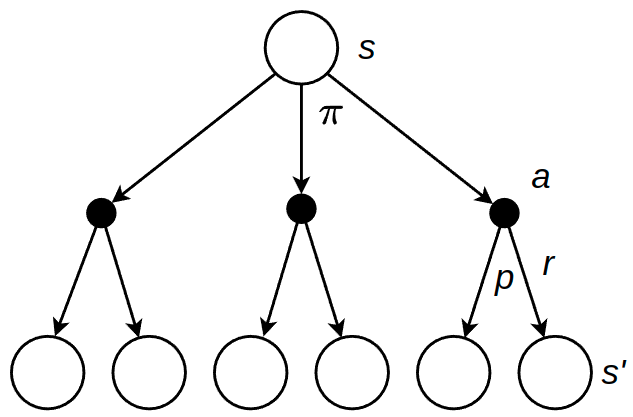
\includegraphics[scale=0.3]{figures/2_RL/2_dp_backup.png}
        \caption{DP methods}
        \label{fig:2_dp_backup}
    \end{subfigure}
    \hfill
    \begin{subfigure}[b]{0.29\textwidth}
        \centering
        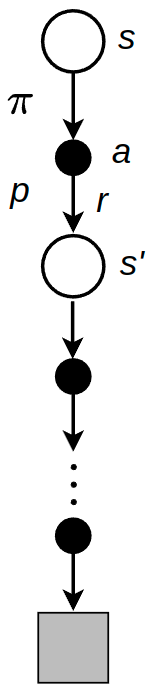
\includegraphics[scale=0.25]{figures/2_RL/2_monte_carlo_backup.png}
        \caption{Monte Carlo methods}
        \label{fig:2_monte_carlo_backup}
    \end{subfigure}
    \caption{The backup diagrams for $V(s)$ for DP and Monte Carlo methods. These diagrams show how information transfers back to a state from its successor states. DP methods update $V(s)$ using information from one-step transitions, while Monte Carlo samples a return $G$ from an entire episode, stopping only at a terminal state. \cite{suttonAndBartoBook}.}
    \label{fig:2_dp_and_monte_carlo_backup}
\end{figure}

By sampling the return, Monte Carlo methods are then able to update their value function $V(S_t)$ -- the expected return for being in a state $S_t$ -- using the sampled return from that state:
\begin{equation}
    V(S_t) \leftarrow V(S_t) + \alpha \, \Big[ G - V(S_t) \Big] \label{eq:2_MonteCarlo_prediction_simplest}
\end{equation}
where $\alpha$ is some step-size parameter.

\subsubsection{TD Value Prediction}
\label{subsubsec:2_TD_value_prediction}
So, to generate an estimate for the value function $V(s)$, we saw that DP methods use one-step updates for $V(s)$ while Monte Carlo methods update $V(s)$ for each state only at the end of an episode. TD methods are similar to Monte Carlo methods since they sample states to update $V(s)$. However, instead of waiting until the end of an episode, TD methods update $V(s)$ at every timestep, similar to DP methods. 
This is seen more clearly in the simplest TD update \cite{suttonAndBartoBook}:
\begin{equation}
    V(S_t) \leftarrow V(S_t) + \alpha \, \Big[ R_{t+1} + \gamma V(S_{t+1}) - V(S_t) \Big] \label{eq:2_TD_prediction_simplest}
\end{equation}
where the value estimates of consecutive timesteps are used as an update rule. The backup diagram of this is shown in \cref{fig:2_td_backup}.
\begin{figure}[hbt]
    \centering
    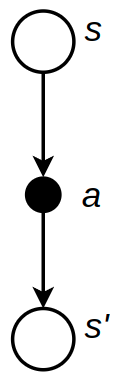
\includegraphics[scale=0.2]{figures/2_RL/2_td_backup.png}
    \caption{Backup diagram for TD methods. Value estimates for state $s$, $V(s)$, are bootstrapped to $V(s')$.}
    \label{fig:2_td_backup}
\end{figure}
The idea of updating an estimate through another estimated value is called \textit{bootstrapping}, where in this case, we say that the current state value estimate $V(S_t)$ is bootstrapped to the next-state value estimate $V(S_{t+1})$. 
Bootstrapping is at the core of DP methods, where we see that the Bellman optimality equations in \eqref{eq:2_V_Bellman} and \eqref{eq:2_Q_Bellman} also follow this bootstrapping form \cite{suttonAndBartoBook}.
The term in the brackets in \eqref{eq:2_TD_prediction_simplest} is also referred to as the \textit{TD-error} $\delta_t$:
\begin{equation}
    \delta_t = R_{t+1} + \gamma V(S_{t+1}) - V(S_t) \label{eq:2_TD_error}
\end{equation}
which will be important later in \cref{subsec:2_actor_critics}. 

To summarise, the point of the update rules for $V^{\pi}(s)$ in equations \eqref{eq:2_policy_iteration_update}, \eqref{eq:2_value_iteration_update}, \eqref{eq:2_MonteCarlo_prediction_simplest} and \eqref{eq:2_TD_prediction_simplest}, is that we wish that our value function reaches the optimal value function $V^{\pi}(s) \rightarrow V^{\pi^*}(s)$, after enough updates. This is similar to any optimisation problem, where we wish to minimise the error between our current value estimate $V^{\pi}(s)$ and some target value estimate $V^{\pi^*}(s)$. For TD learning, this error is the TD-error \eqref{eq:2_TD_error}, where the target value is the estimate $R_{t+1} + \gamma V(S_{t+1})$, which exploits the recursive nature of the optimal value function given by the Bellman optimality equations in \eqref{eq:2_V_Bellman}, similar to DP methods. For Monte Carlo methods, we can see that the target value for the expected return $V(s)$ is the sampled return $G$ in \eqref{eq:2_MonteCarlo_prediction_simplest}; and since the sampled return $G$ is not an estimate per se, Monte Carlo methods also do not bootstrap.


\subsection{Exploration versus Exploitation}
\label{subsec:2_exploration_vs_exploitation}
Now that we have seen how agents can learn optimal value functions, it is important to specify that model-free methods more commonly rely on learning the action-value function $Q(s, a)$ instead of $V(s)$. The reason is that learning the Q-function allows the agent to solve the reinforcement learning problem by simply selecting the action with the greatest return, without needing to consider possible next-states or the dynamics of the environment \cite{suttonAndBartoBook}.

However, learning the Q-function in sampling-based methods requires that we specify what action to take in our target Q-function estimate.
Unlike model-based methods, sampling-based methods require an adequate exploration of all actions $a \in \mathcal{A}(s)$ in a given state $s$ in order to achieve an accurate state-action value $Q^{\pi}(s, a)$ for that state. However, the goal of the reinforcement agent is also to maximise its expected return, which means to \textit{greedily} choose actions $a$ as shown in \eqref{eq:2_dp_optimal_policy} in value iteration. The question of whether and when an agent should exploit its current knowledge of the value of actions, or attempt to explore actions that might yield a higher return in the long run, is referred to as \textit{exploration versus exploitation} \cite{suttonAndBartoBook}.
For TD learning, handling this question brings us to the topic of \textit{on-policy} and \textit{off-policy} methods.



\subsection{On-policy and Off-policy methods*}
\label{subsec:2_on-policy_off-policy_methods}
Generally speaking, the difference in on-policy and off-policy methods lies in the action-value function update step, specifically how the current action value estimate is bootstrapped to the action value estimates of consecutive states. 
The best way to visualise this is through the use of an example, where we will look at two fundamental methods, \textit{SARSA} \cite{suttonAndBartoBook} and \textit{Q-learning} \cite{watkins1992QLearning}: \\[5mm]
\textbf{On-policy} -- The update step for SARSA:
    \begin{equation}
        Q^\pi(S_t, A_t) \leftarrow Q^\pi(S_t, A_t) + \alpha \, \Big[
        R_{t+1} + \gamma Q^\pi(S_{t+1}, A_{t+1}) - Q^\pi(S_t, A_t)
        \Big] \label{eq:2_SARSA}
    \end{equation}
\textbf{Off-policy} -- The update step for \textit{Q}-learning:
\begin{equation}
    Q^\pi(S_t, A_t) \leftarrow Q^\pi(S_t, A_t) + \alpha \, \Big[
    R_{t+1} + \gamma \max_a Q^\pi\,(S_{t+1}, a) - Q^\pi\,(S_t, A_t) 
    \Big] \label{eq:2_Qlearning} \vspace{1mm}
\end{equation} 
In both cases, the policy $\pi$ is an arbitrary policy, e.g. choosing a random action with $\epsilon$ probability and the max action with probability $1-\epsilon$ ($\epsilon$-greedy).
SARSA is dubbed an \textit{on-policy} algorithm as the next state-action value estimate is based on \textit{exactly the same policy} as the agent's current one. This means that when updating the current state-action value pair, the value of the next state-value pair is evaluated to be the expected return $Q^\pi(S_{t+1}, A_{t+1}$ from a state $S_{t+1}$ after taking an action $A_{t+1}$ under the \textit{same} \textit{behaviour} policy $\pi$. It can also be said that the \textit{target policy} for on-policy methods is the same as its current policy, if we think of the update as an error between the current and target policies.

In contrast, \textit{Q}-learning uses an update step of $\max_a Q^\pi\,(S_{t+1}, a)$, while its behaviour policy could be for example, $\epsilon$-greedy. As a result, the actions chosen in the subsequent states will always be \textit{greedy} choices and \textit{not actions chosen under its behaviour policy} $\pi$, which was only greedy with probability $1-\epsilon$ ($\epsilon$-greedy).
So, methods that bootstrap current value estimates (under behaviour policy $\pi$) to estimates derived from a \textit{different} target policy $\pi'$ are referred to as off-policy methods. In these cases, the behaviour policy is often denoted as $\beta$, while the target policy can be denoted as $\pi(a|s)$ if stochastic or $\pi(s)$ if deterministic.

Going back to the question of exploration versus exploitation, the result of updating $Q^\pi(S_t, A_t)$ with a greedy target policy, like in off-policy \textit{Q}-learning, is that the learned policy is more likely to suggest taking actions that follow this ``optimal'', greedy trajectory, rather than exploring the action space more in order to find another more optimal approach. 
Off-policy methods try to overcome this by explicitly choosing a behaviour policy $\beta$ that is exploratory by nature, for example, a random policy or one with added noise. The after-effect of choosing a highly exploratory action is that many obvious ``bad'' actions could be taken -- unnecessarily slowing learning. This is especially true when state and action spaces are large, as we want the agent to explore actions close to an optimal trajectory rather than waste time exploring actions far from the optimal solution. 
In contrast, on-policy methods avoid this issue by not updating estimates with greedy strategies in the first place, though they still have the potential to suffer from insufficient exploration. A reverse problem for on-policy methods is that, by definition, they do not have a behaviour policy that they can specify explicitly. Hence, they are limited to defining a target policy that incorporates some degree of randomness so as to prevent converging to some locally optimal solution.

\subsection{An Extension to Continuous Control*}
\label{subsec:2_an_extension_to_continuous_control}

So far, the methods that we have seen have only been applicable to MDPs; \textit{tabular solution methods} like DP, Monte Carlo, and TD learning only work in environments with a relatively small, finite set of \textit{discrete} states and actions \cite{suttonAndBartoBook}. However, for most of the interesting control problems in cybernetics, we deal with \textit{continuous} state and action spaces. In these problems, a simple question of how one should represent the state space $\mathcal{S}$ or the action space $\mathcal{A}(s)$ can quickly become challenging. 
For example, the discretisation of these continuous spaces has a severe limitation: namely the \textit{curse of dimensionality}, where the number of both state and action combinations grows exponentially by the number of degrees of freedom \cite{BellmanDreyfus1962Book}. Thus, methods that rely on finding the maximum action in order to update its action-value function, such as in \eqref{eq:2_Qlearning} in Q-learning, will then require an iterative optimisation process at each step due to the large set of possible actions \cite{DDPG}, which is impractical if not infeasible. 

As a result, these high-dimensional continuous state and control problems strictly restricts us to finding an only \textit{approximate} solution for the policy and value functions, which motivates the use of \textit{approximate solution methods} -- methods that focus on \textit{generalisation through function approximation} \cite{suttonAndBartoBook}.
This restriction is also a motivation for the relevance of \textit{policy search}, as policies require less representational power than a value function approximation \cite{BagnellPolicySearch2003} and can frankly, just be simpler to approximate \cite{suttonAndBartoBook}.
So, finding an adequate parametrisation of these functions has also become a key focus in reinforcement learning in recent years.
Fortunately for us, there has been a clear parametrisation of choice for both value function and policy in recent years, through the use of \textit{neural networks} (NNs) as universal function approximators, initially inspired by the success of \textit{Deep Q-Networks} (DQNs) \cite{DQN} and later, \textit{Deep Deterministic Policy Gradients} (DDPG) \cite{DDPG}.\todo{maybe talk about DQN and DDPG, instability to train}
In the literature, we refer to all methods that learn a parametrised policy $\pibt$, through the gradient of some performance measure $J(\bt)$ with respect to parametrised policy parameters $\bt$ as \textit{policy gradient methods}. \todo{change intro to accommodate for this intermediate subsection} 

\subsection{Policy Gradient Methods}
\label{subsec:2_policy_gradient_methods}
Policy gradient methods are a form of policy search, where we have a vector of $d$ parameters $\bt \in \mathbb{R}^d$ that parametrises our policy $\pi$:
\begin{equation}
    \pibt = P \, ( \, A_t = a \, | \, S_t = s, \bt_t = \bt)
\end{equation}
Policy gradient methods have a goal of optimising a certain objective function $J(\bt)$, with respect to these parameters $\bt$. A typical objective function could be the expected return at a particular state under the parametrised policy $\pi_{\bt}$, or simply the value function \eqref{eq:2_value_function}:
\begin{equation}
    J(\bt) = V^{\pi_{\bt}}(s) \label{eq:2_2_JvalueFunc}
\end{equation}
As the objective function also depicts a performance measure that we wish to maximise, rather than a loss, we aim to maximise it through \textit{gradient ascent} \cite{suttonAndBartoBook}:
\begin{equation}
    \bt_{t+1} = \bt_t + \alpha \widehat{\nbt \, J(\bt_t)} \label{eq:2_2_gradientasc}
\end{equation}
Here, the gradient term of the objective $J(\bt)$, with respect to the policy parameters $\bt_t$, is represented by $\widehat{\nabla_{\bt} \, J(\bt_t)}$ and is a stochastic estimate. So, we describe all methods that use a parametrisation of the policy $\pi$ as policy gradient methods, and what normally varies is how we define the objective function $J(\bt)$.

If we use the value function as the performance measure as in \eqref{eq:2_2_JvalueFunc}, we obtain the key result in policy gradient methods, the \textit{policy gradient theorem}, where we can express the gradient of the objective function, with respect to the policy parameters $\bt$ as \cite{suttonAndBartoBook}:
\begin{align}
    \nbt J(\bt) &\propto \sum_s p(s) \sum_a Q^{\pi} (s,a) \, \nbt \pi_{\bt} \, (a \, | \, s) \label{eq:2_2_policyGradient1} \\
    &= \E_{\pi,\, S_t \sim p(s)} \left[\sum_a Q^{\pi_{\bt}} (S_t,a) \, \nbt \pi_{\bt} \, (a \, | \, S_t) \right] \label{eq:2_2_policyGradient2}
\end{align}
where $p(s)$ is the \textit{on-policy state distribution}, as mentioned in \cref{subsec:2_MDPs}, which represents the probability distribution of states under $\pi$, and can be thought of as the fraction of time spent at a state $s$, where $\sum_s p(s) =1$ \cite{suttonAndBartoBook}.
Then, as $p(s)$ serves as a weighting for states $s$, we see that \eqref{eq:2_2_policyGradient1} can be simplified to just an expectation in \eqref{eq:2_2_policyGradient2}.

The policy gradient theorem in \eqref{eq:2_2_policyGradient2} is a central result in reinforcement learning because it summarises how a parametrised policy $\pibt$ can be optimised without the need for any model information.
Intuitively, the policy performance should depend on both the probability of actions and the distribution of states for which the actions are taken in, i.e. the state distribution $p$ -- though this is impossible to know in a model-free setting. Nevertheless, we see that the gradient does not depend on the state distribution $p$ but only on the expected return and the gradient of the policy parameters. 

As a result, algorithms have been derived that attempt to estimate this expectation through a sample-based approach, though a question for policy gradient methods has been on finding a good sample for $Q^{\pi_{\bt}} (s, a)$ \cite{DPG}. The issue is that the sampled returns for episodes can vary greatly, leading to high-variance updates in the policy space that can lead to convergence difficulties. This makes it difficult to simply use the sampled return as an estimate for $Q^{\pi_{\bt}}(s,a)$ \cite{suttonAndBartoBook}. Thus, as an extension to mend this problem, we have actor-critic methods.


\subsection{Actor-Critics*}
\label{subsec:2_actor_critics}

Actor-Critic methods follow the same idea as policy gradient methods but also include a parametrisation of the action-value function $Q(s, a)$. In other words, these methods aim to concurrently learn a policy $\pi(a\,|\,s)$ and the action-value function $Q(s,a)$. 
The \textit{actor} refers to the parametrisation of the policy $\pi(a\,|\,s)$ through $\bt$, while the \textit{critic} refers to the parametrisation of the action-value function $Q(s,a)$ through a vector $\bw$ \cite{suttonAndBartoBook}. The critic could also parametrise the value function $V(s)$ instead, as in PPO \cite{PPO}.

\subsubsection{Updating the Actor Parameters}
To make use of this critic, we incorporate it into the update step for the actor in the form of a \textit{baseline}, $b(s)$. By comparing the estimate to this baseline, we can reduce the variance of the actor updates significantly and beneficially \cite{suttonAndBartoBook}. A simple baseline can be added to the gradient as so:
\begin{equation}
    \nbt J(\bt) \propto \sum_s p(s) \sum_a \Big(Q^{\pi_{\bt}} (s,a) - b(s) \Big) \, \nbt \pi_{\bt} \, (a \, | \, s) 
\end{equation}
However, to get this expression into the form we desire, we have to simplify the expression into just an expectation, similarly to \eqref{eq:2_2_policyGradient2}.
This is done by adding the missing weight for each actions, which is the stochastic policy $\pi(a|s)$:
\begin{align*}
    \nbt J(\bt) &= \E_{\pi, \, S_t \sim p(s)} \left[\sum_a \pi_{\bt} \, (a \, | \, S_t) \, \Big(Q^{\pi_{\bt}} (S_t,a) -b(s) \Big)\, \nbt \frac{\pi_{\bt} \, (a \, | \, S_t)}{\pi_{\bt} \, (a \, | \, S_t)} \right] \\
    &= \E_{\pi, \, S_t \sim p(s), \, A_t \sim \pi} \left[\Big(Q^{\pi_{\bt}} (S_t,A_t) -b(s)\Big)\, \frac{\nbt \pi_{\bt} \, (A_t \, | \, S_t)}{\pi_{\bt} \, (A_t \, | \, S_t)} \right] \\
    &= \E_{\pi, \, S_t \sim p(s), \, A_t \sim \pi} \left[\Big(G_t -b(s)\Big)\, \frac{\nbt \pi_{\bt} \, (A_t \, | \, S_t)}{\pi_{\bt} \, (A_t \, | \, S_t)} \right] \numberthis \label{eq:2_montecarlo_actor_update}
\end{align*}
Here, $G_t$ is the return with the same expectation as the $Q^{\pi_{\bt}} (S_t,A_t)$ value. Yet, two observations should be made to this result: first, this gradient assumes we can sample the return (like a Monte Carlo method), and second, the baseline is strictly not a critic in the fact that it does incorporate information from the consecutive time steps \cite{suttonAndBartoBook}. Thus, there is one more step that has to be taken in order to achieve the result we desire. To both bypass the need to sample the return and be considered an actor-critic method, actor-critics borrow ideas from TD learning by bootstrapping its action value estimate to the next-state action value estimate:
\begin{gather}
    \nbt J(\bt) = \E_{\pi, \, S_t \sim p(s), \, A_t \sim \pi} \left[ \delta_t \,
    \frac{\nbt \pi_{\bt} \, (A_t \, | \, S_t)}{\pi_{\bt} \, (A_t \, | \, S_t)} \right]  \label{eq:2_actor_grad} \\[5mm]
    \delta_t = R_{t+1} + \gamma Q_{\bw}^{\pi_{\bt}}(S_{t+1}, A_{t+1}) - Q^{\pi_{\bt}}_{\bw}(S_t, A_t) \vspace{5mm} \label{eq:2_}
\end{gather}
where we recognise $\delta_t$ as the TD error from \eqref{eq:2_value_td_error}. So finally, the actor update can be represented as:
\begin{equation}
    \bt_{t+1} = \bt_t + \alpha^{\bt} \delta_t \frac{\nbt \pi_{\bt} \, (A_t \, | \, S_t)}{\pi_{\bt} \, (A_t \, | \, S_t)} \label{eq:2_actor_update}
\end{equation} 

\subsubsection{Updating the Critic Parameters}
As for the critic, we aim to take a step in the direction that reduces the error between the approximate value $Q^{\pi_{\bt}}(s, a \,| \,\bw)$ and the true value $Q^{\pi_{\bt}}(s,a)$. This is known as the \textit{Mean Squared Value Error}, $\overline{VE}\,$  \cite{suttonAndBartoBook}:
\begin{equation}
    \overline{VE}\,(\bw)= \E_{\pi, \, S_t \sim p(s), \, A_t \sim \pi} \Big[ 
    \big( Q^{\pi_{\bt}}(S_t, \, A_t) - Q^{\pi_{\bt}}_{\bw}(S_t, \, A_t) \label{eq:2_critic_loss} \big)^2
    \Big]
\end{equation}
The way forward is quite similar to the value prediction methods we have seen before, where we have to choose how to represent our target $Q^{\pi_{\bt}}(s,a)$. We can choose this to be the Monte Carlo sample $G_t$, though we instead choose it to be the bootstrapping target $R_{t+1} + \gamma Q_{\bw}^{\pi_{\bt}}(S_{t+1}, A_{t+1})$.

Then, we can minimise this error through stochastic gradient descent, where we take the gradient of the $\overline{VE}$ with respect to the parameters $\bw$. This gives us the update rule in \textit{Semi-gradient TD(0)}:
\begin{gather}
    \bw_{t+1} \leftarrow \bw_{t} + \alpha^{\bw} \delta_t \nabla_{\bw} Q_{\bw}^{\pi_{\bt}} (S_t, \,A_t) \label{eq:2_critic_update} \\[3mm]
    \delta_t = R_{t+1} + \gamma Q_{\bw}^{\pi_{\bt}}(S_{t+1}, \,A_{t+1}) -Q_{\bw}^{\pi_{\bt}} (S_t, \,A_t) 
    \label{eq:2_value_td_error}
\end{gather}
with $\delta_t$ as the TD-error. So, by using a ``bootstrapping critic'', we can introduce a bias -- injecting information based on the assumption that our critic should be in a value function form, i.e. it follows a recursive nature with optimal form as \eqref{eq:2_Q_Bellman}. Moreover, this allows for every-step updates as mentioned in \cref{subsec:2_TD_learning}, and, ``typically enables significantly faster learning'' of the value function \cite{suttonAndBartoBook}. 

Lastly, compared to Monte Carlo policy gradient methods that sample the return, we also see that by taking the TD-error in the actor gradient, the same benefit of reduced variance of gradient updates and accelerated learning is applied \cite{suttonAndBartoBook}.


\subsection{Proximal Policy Optimisation*}
\label{subsec:2_PPO}

In light of the advancements within deep reinforcement learning from \cite{DQN} and \cite{DDPG}, a new family of methods was developed to curb the problem of instability and divergence when training agents using NNs. These are called \textit{trust-region} based policy optimisation methods, stemming from Trust-region Policy Optimisation (TRPO) \cite{TRPO}.
PPO \cite{PPO} is heavily inspired by this, where the overarching idea is that in order to maintain stability in training, the new, updated policy should be within a specific \textit{trust-region} of the old policy, hence the name \textit{proximal} policy.
As for its other characteristics, PPO is also a model-free, on-policy and actor-critic method, parametrising a stochastic policy $\pi(a\,|\,s)$ and a value function $V(s)$. Finally, it introduces a uniquely defined objective function to optimise this.

\subsubsection{The Advantage Function}
Earlier, we defined the policy gradient in \eqref{eq:2_actor_grad}. This can be implemented in practice as:
\begin{equation}
    \widehat{\nbt J_t(\bt)} = \hatE \left[ 
    \frac{\nbt \pibt}{\pibt} \: \hatA (s, a) 
    \right] \label{eq:2_ppo_actor_grad}
\end{equation}
where $\hatE$ represents the empirical average over a finite batch of samples of actions $a$ and states $s$. Also, we introduce a colloquial term $\hat{A}$, called the \textit{advantage} function $A : \mathcal{S} \times \mathcal{A} \rightarrow \mathbb{R}$, that represents how well an action did compared to some \textit{baseline} estimate:
\begin{equation}
    \hat{A}\,(s ,a) = \underbrace{Q\, (\,s,\, a\,)}_{\text{discounted return}} - \quad \underbrace{V_{\bt}\,(\,s\,)}_{\text{estimate}} \label{eq:2_ppo_advantage}
\end{equation}
The baseline in this case is the parametrised value function $V_{\bt}$. Note that the first term shows the rewards that was actually received, while the second is an estimate of what we expected to receive in that state -- the critic. Hence, the advantage gives an idea of whether the action performed was better or worse than expected by the critic. 

\subsubsection{PPO-Clip Objective}
PPO ensures that the new policy is close to the old one by using one of two tricks: clipping or an adaptive KL divergence penalty term. Primarily, the one that is used is the \textit{clipped surrogate objective} version of PPO, which is also used in this thesis. In this version, the authors prevent substantial changes to the policy parametrisation by basically flattening the policy objective function to a certain maximum value. To visualise this, we can look at the novel objective function used.

PPO takes the surrogate objective function used by TRPO, whose gradient is equivalent to \eqref{eq:2_ppo_actor_grad}:
\begin{equation}
    J_t(\bt) = \hatE \left[ 
    \frac{\pibt}{\pibtold} \: \hatA (s, a) 
    \right]
    = \hatE \left[ 
    r_t(\bt) \: \hatA (s, a) 
    \right] \label{eq:2_trpo_actor_objective}
\end{equation}
and clips it by a maximum value bounded by a hyperparameter $\epsilon$ to obtain the \textit{actor objective function}:
\begin{equation}
    J_t^{CLIP}(\bt) = \hatE \left[ \min\,(
    r_t(\bt) \: \hatA (s, a), \, \text{clip}\, ( r_t(\bt), 1-\epsilon, 1+\epsilon) \; \hatA(s,a)
    \right]
    \label{eq:2_ppo_clipped_objective}
\end{equation}
This clipping aims to remove the incentive from deviating more than $\epsilon$ away from the old policy \cite{PPO} and can be visualised in Figure \ref{fig:2_ppo_actor_clip}. Also, the ratio $r_t(\bt) = \frac{\pibt}{\pibtold}$ can be understood as the change in probability of selecting actions compared to the old policy, $\pibtold$, such that $r_t(\bt_{\text{old}}) = 1$.
\begin{figure}[htb]
    \centering
    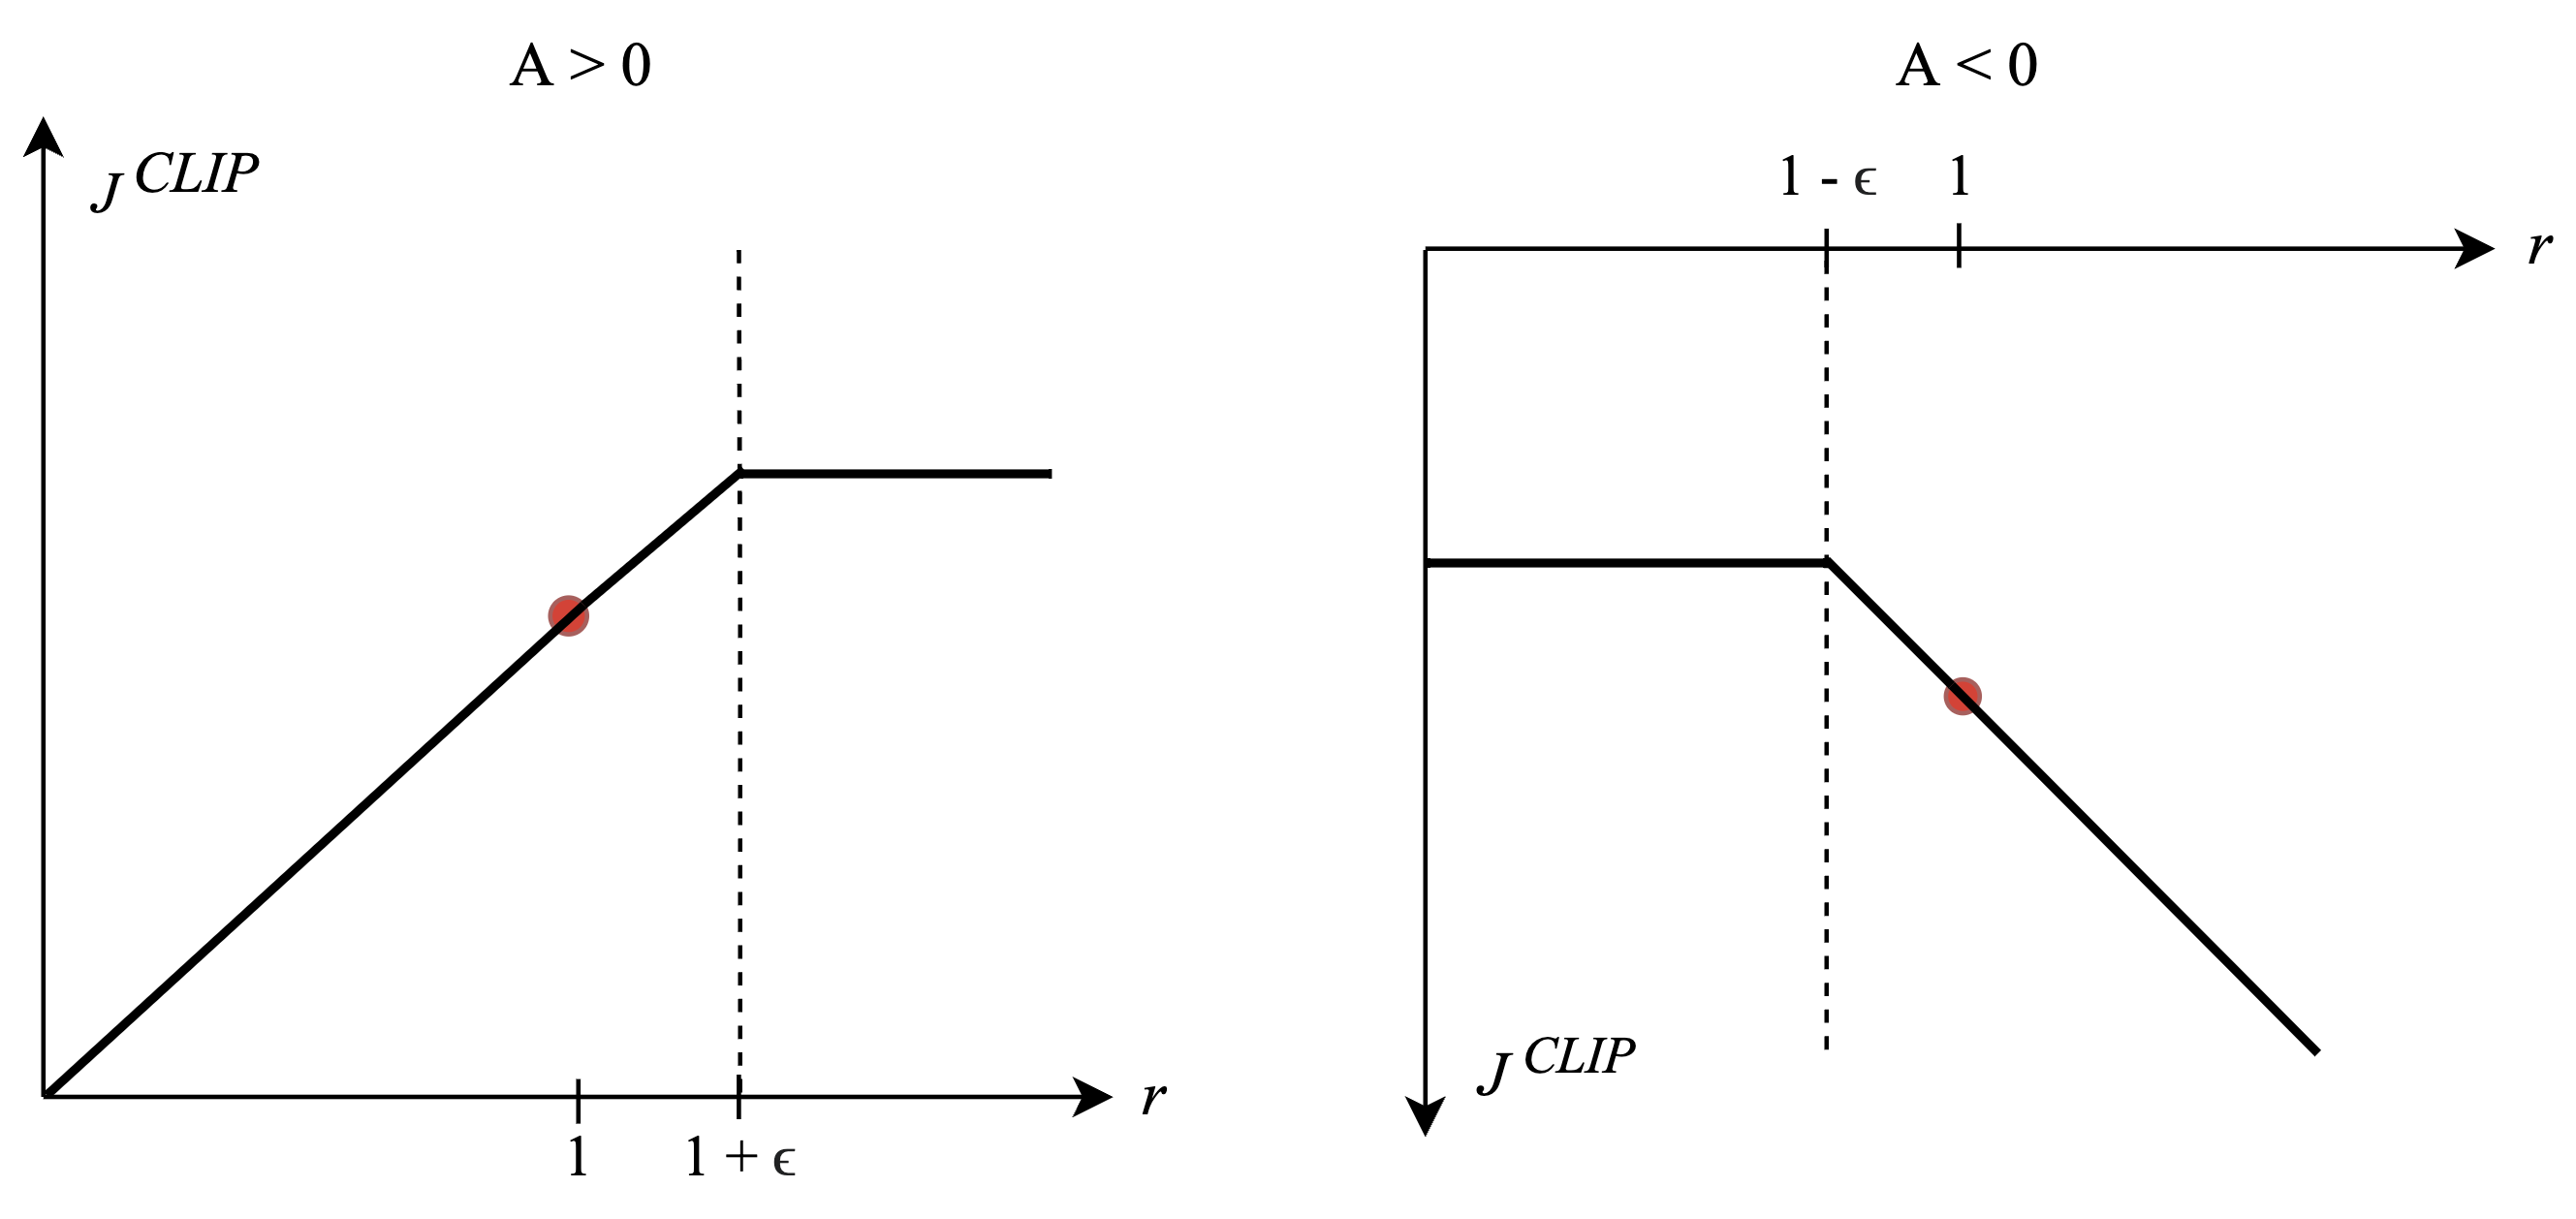
\includegraphics[width=0.8\textwidth]{figures/2_RL/2_ppo_actor_clip.png}
    \caption{Visualising the clipped surrogate objective function for positive and negative advantages $A$. The figure is recreated from the original paper \cite{PPO}.}
    \label{fig:2_ppo_actor_clip}
\end{figure}

The way to understand the clipped surrogate objective is to first remember that we are performing gradient ascent in the objective function, w.r.t. the policy parameters $\bt$. This means that we essentially choose the direction in which $r_t(\bt)$ should move in \eqref{eq:2_ppo_clipped_objective} and Figure \ref{fig:2_ppo_actor_clip}. When the agent performs better than expected, i.e. the advantage is positive, we wish to increase the probability of doing those actions again, which is equivalent to increasing $r_t(\bt)$. So, we adjust the parameters $\bt$ such that the probability ratio $r_t(\bt)$ moves to the right. However, since we are taking the minimum and the objective is clipped at $1+\epsilon$, there is no added benefit of increasing $r_t(\bt)$ beyond this clipped point. Similarly, when the agent performs worse than expected, i.e. the advantage is negative, we wish to lower the probability of those actions happening again, which is equivalent to reducing the probability ratio $r_t(\bt)$. Again, since we clip the value at $1-\epsilon$ and the objective function is taking the minimum, there is no benefit of decreasing $r_t(\bt)$ beyond the clipped point. Therefore, by aiming to maximise the performance objective in \eqref{eq:2_ppo_clipped_objective} by gradient ascent, the authors manage to prevent the new policy from deviating too far from the old one, as seen by $r_t(\bt)$ being discouraged from moving beyond $[1-\epsilon, 1+\epsilon]$. 


\subsubsection{Actor-Critic Structure}
With the key idea from PPO presented, we can delve into the actor-critic structure of PPO. As shown above, the policy gradient is based on the advantage term $\hatA$. As a result, PPO uses a parametrisation of the value function $V(s)$ as a critic, so to produce an estimate for the advantage $\hatA$ in \eqref{eq:2_ppo_advantage}.
Similarly to before \eqref{eq:2_critic_loss}, the parametrised value function can be optimised by minimising the mean squared value error $\overline{VE}$:
\begin{equation}
    J_t^{VF}(\bt) = \E_t \Big[(V_{\bt_t}(s) - V_t^{\text{targ}})^2\Big] \label{eq:2_ppo_critic_loss}
\end{equation}
where the target value function $V_t^{\text{targ}}$ that was implemented in the code of \cite{PPO} is defined as:
\begin{equation}
    V_t^{\text{targ}} = R_t + \gamma V_{\bt_t}(s')
\end{equation}
Lastly, there is an entropy term $S[\pi_{\bt}](s)$ that is also added to the objective function, which serves as an exploration term. 

So combined, the overall objective function for PPO with the actor objective function in \eqref{eq:2_ppo_clipped_objective}, critic loss in \eqref{eq:2_ppo_critic_loss} and entropy term, is:
\begin{equation}
    J_t^{CLIP+VF+S}(\bt) = \hatE \Big[
    J_t^{CLIP}(\bt) + c_1 J_t^{VF}(\bt) + c_2 S[\pi_{\bt}](s)
    \Big],   \label{eq:2_ppo_full_objective}
\end{equation}
where $c_1$ and $c_2$ are coefficients. PPO also assumes that some automatic differentiation software is used, such that the software is able to keep track of how each objective function is computed in order to backpropagate the gradients appropriately. This also allows PPO to simply combine the objective functions like above.

In the PPO implementation, the parameters $\bt$ characterise the whole actor-critic model, though ``under the hood'' it can also be two different NNs that receive their own respective gradients, such as in \cite{LearningWalkMassivelyParallel} or \cite{AMPMotionPriors}. However, they have made this generalisation in the case where parameter-sharing is desired, where the ``bottom'' hidden layers are the same, and the network heads are different -- such as in this thesis, which will be discussed briefly in \cref{subsec:5_MLP_architecture}. Moreover, since the actor is parametrising a stochastic policy, the head of the actor network outputs the parameters of the policy distribution, which for continuous cases is normally chosen to be a Gaussian distribution.

Furthermore, one of the things to keep in mind is that PPO is also an on-policy algorithm. This means that when the agent is sampling experiences, these samples are gathered under its current policy $\pibt$. Hence, in its actor-critic implementation, a sample \textit{trajectory} $\boldsymbol{T}$ is first collected under a policy $\pibt$ for $T$ timesteps before updates are made to the actor and critic parameters $\bt$. This means after $T$ timesteps, we have also received the rewards for each timestep and can compute the advantage estimates $\hatA$ for every timestep $t = 1, 2, ..., T$.
Then, when we are optimising the performance objective, we have the opportunity to define how many epochs $K$ were in that trajectory of size $T$, which means that we can specify how many gradient updates to do using the same batch of experiences. After the updates are completed, we discard this trajectory of experiences and begin sampling a new one to ensure that the new experiences occur under the new policy $\pi_{\bt}$. 
\begin{figure}[ht]
    \centering
    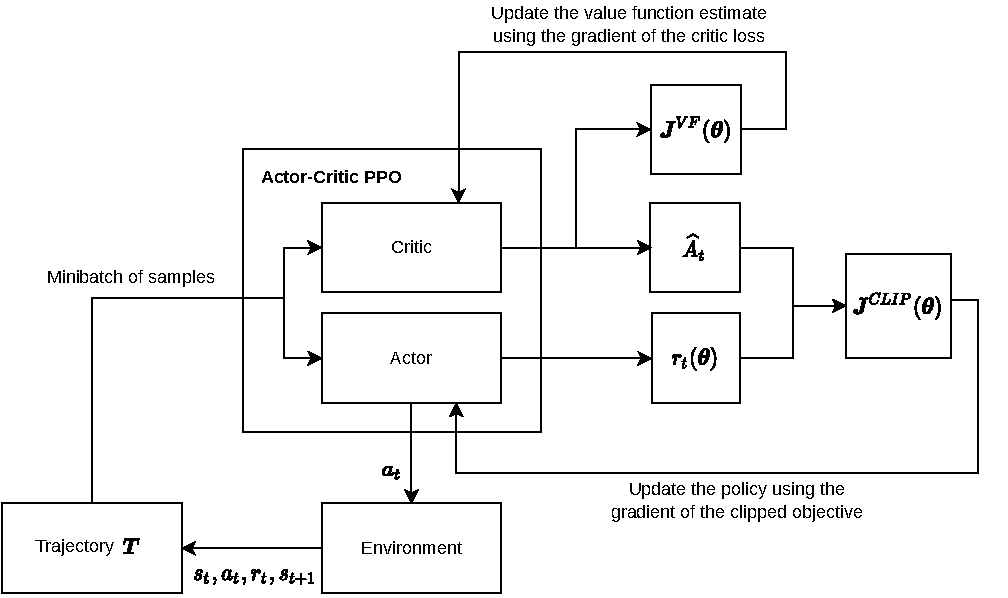
\includegraphics[width=0.95\textwidth]{figures/2_RL/2_ppo_overview.pdf}
    \caption{An overview of how the actor and critic networks are updated in PPO. Once the loss terms are calculated, the gradients $\nabla J_t^{CLIP}(\bt)$ and  $\nabla J_t^{VF}(\bt)$ are used to update the actor and critic respectively.}
    \label{fig:2_ppo_overview}
\end{figure}
Conceptually, we can view the whole update process in Figure \ref{fig:2_ppo_overview}. Here, we first see that a trajectory is sampled based on the current policy given by the actor before the loss terms are calculated. Finally, the gradient of the objective function w.r.t. to the actor and critic weights is used to update the actor and critic networks.

\subsubsection{Summary}
PPO can solve a vast variety of continuous reinforcement learning problems by being a model-free, actor-critic method and using neural networks as function approximators. It is also an on-policy method, meaning the sampled trajectory of experiences is collected under its current policy $\pibt$. The algorithm is able to achieve state-of-the-art performances through its adaptation of the trust-region based method, TRPO, where the idea is to take the largest possible step in the right direction while ensuring that the new policies, after an update, stay close (or are \textit{proximal}) to the old one. In turn, as stated in TRPO \cite{TRPO}, this should guarantee a monotonic improvement of the policy.

In terms of implementation, it is relatively simple compared to its counterpart, TRPO. It uses a clipped surrogate objective to define its proximal policy aim rather than a hard constraint that requires second-order methods to optimise. Also, as it assumes we are using an automatic differentiation software, we can combine the objective functions for both the policy and the value function parametrisations, where the software is able to keep track of how to compute the gradients (perform backpropagation) for the respective parameters.

Also, since it is on-policy, it retains its high data efficiency and reliable performance. This is particularly significant for problems with high-dimensional state and action spaces since the agent can focus on exploring actions along its current policy instead of calculating less gradients from actions in states that are very uncommon. This is also why it is more data-efficient, as it can converge to an optimal behaviour faster.

Though conversely, since PPO is on-policy, the \textit{overall} degree of exploration is based mainly on its stochastic policy $\pibt$, with the exception of the entropy term. As discussed in \cref{subsec:2_an_extension_to_continuous_control}, this means that the agent may suffer from a lack of exploration if its policy does not incorporate some degree of randomness. Yet, by the nature of optimisation, PPO will progressively increase probabilities of doing ``good'' actions and decrease probabilities of doing ``bad'' ones, based on its estimate of advantage and value function. This means that over time, the agent will exploit the environment more, irrespective of how accurate its estimate of the policy and value function is, and could become trapped in a local optimum. 
